%Mathdocs. MG changed some things, see end of document. This is the master copy, altered on 8/28/2022 for tkzEuclide
\documentclass[addpoints]{amsart} 
%\documentclass{tglat2e}%%   tglat calls the Class of our Journal.
\parskip 5pt
\textwidth 5.5in
%\linespread{1.2}
%\hoffset-.8truein
%\vsize10truein
%For large fonts, use \tiny, \scriptsize, \footnotesize, \Large, \LARGE, \huge, \Huge.

%\usepackage{gensymb} %for degree symbol
\usepackage{pgf, tikz} %8/26/22 I put in the pgf for Euclide
%\usepackage{tikzsymbols} %for emoticons! Call with \Smiley, \Sadey, \Neutrey, and put [2.0] to make it twice as big. see lists.
\usepackage{tikz-cd} %Commutative Diagrams. Use \[\begin{tikzcd} .. \end{tikzcd}\] You can make: A \arrow[hook]{r} & B
\usetikzlibrary{angles,arrows.meta,automata,backgrounds,calc,decorations.markings,decorations.pathreplacing,intersections,patterns,positioning,quotes} %For background figures, use \begin{scope}[on background layer] ... \end{scope}
\usetikzlibrary{shapes} %For polygon nodes, see http://www.texample.net/tikz/examples/node-shapes/
\usepgflibrary{shapes.geometric}
\usepackage{tkz-euclide} 
%Needed to resolve conflict between tkz-euclide and thmtools, see https://tex.stackexchange.com/questions/456029/thmtools-and-tkz-euclide-conflict
%\usetkzobj{all}
%\usepackage{thmtools}
\usepackage{etoolbox}
\usepackage{url}
\usepackage{hyperref}


\usepackage{mdframed} %\begin{mdframed}[backgroundcolor=green!10,linewidth=1pt] makes a colored box around an enumerate, etc.
\usepackage{pgfplots}
\pgfplotsset{width=10cm,compat=1.9}
\usepackage[export]{adjustbox}
\usepackage{caption}
\usepackage{subcaption}
\usepackage{wrapfig}
%See sharelatex.com
\usepackage{graphicx}
\usepackage{mathtools}  %This allows the \begin{bmatrix*} environment, and a [r] [l], or [c] which aligns the entries!
%See sharelatex.com
\usepackage{amsthm,thmtools} %This allows boxed theorem-like environments, see \declaretheorem as below
%I removed this 8/26/2022 trying to fix euclide, as I heard there was a conflict.
\usepackage{relsize} %for a cup product $\mathsmaller\cup$

\usepackage{fdsymbol} %Or {mnsymbol}
%\usepackage{amssymb, latexsym, amsmath} %is what we had before fdsymbol%, makeidx}
%\makeindex

\usepackage{amsmath,systeme} %this is for systems of equations. 
%You use \begin{equation*}\systeme{<put in system, separating equations with a comma>}\end{equation*}. 
%If you want to get rid of the delimiter, use \sysdelim..\systeme{ } instead.

\usepackage{fancyhdr} %headers and footers. On the document, put \pagestyle{fancy} before begin{document}, then use \rhead{Cal Poly}, \chead{\bf Math 241}, \lhead{Brussel}. Or, \fancyhead[L]{Math 483/560}, \fancyhead[R]{bbbbbbbbbbbbbbbbbb}, \fancyhead[C]{Structure}, then \begin{document}\thispagestyle{fancy} <- If you want the first page as well.

%FONTS:
\usepackage{courier}
%call it up with \texttt.  It gives an equally spaced courier font.
\input ArtNouvc.fd
\newcommand*\initfamily{\usefont{U}{ArtNouvc}{xl}{n}} %Fancy all caps. Call it with {\initfamily <text>}
\input Starburst.fd
\newcommand*\starinitfamily{\usefont{U}{Starburst}{xl}{n}}

\usepackage[all,cmtip]{xy}
%See website http://en.wikibooks.org/wiki/LaTeX/Creating_Graphics#XY-pic
%http://www.tug.org/pracjourn/2006-4/blaga/blaga.pdf

\usepackage{enumerate}
%Follow the usual \begin{enumerate} with [I] for roman numerals, and [(a)] for alphabetic symbols.
\usepackage{mdwlist}

%I blocked this when I put in tikz, because of a color clash.
%\usepackage[usenames, dvipsnames]{color}
%See website http://people.oregonstate.edu/~peterseb/tex/samples/color-package.html for
%a list of the many color options.  Or, http://en.wikibooks.org/wiki/LaTeX/Colors
%To invoke, use {\color{red}<text>}
%To make a new color, use \definecolor{orange}{rgb}{1,0.5,0}  Here rgb is red green blue.

%%%%% from Asher
\usepackage{mathrsfs} %nice script font
%%% UV - changes in header: %'d \usepackage{mathabx}, \def\divides, \def\notdivides.
%\usepackage{mathabx} % get \notdivides

\usepackage[OT2,T1]{fontenc}
\DeclareSymbolFont{cyrletters}{OT2}{wncyr}{m}{n}
\DeclareMathSymbol{\Sha}{\mathalpha}{cyrletters}{"58}



\theoremstyle{plain}
\newtheorem{Theorem}[subsubsection]{Theorem}
\newtheorem{Lemma}[subsubsection]{Lemma}
\newtheorem{Corollary}[subsubsection]{Corollary}
\newtheorem{Proposition}[subsubsection]{Proposition}
\newtheorem{Notation}[subsubsection]{Notation}
\newtheorem{Definition}[subsubsection]{Definition}
%\newtheorem{Equation}[subsubsection]{Equation}
%the [equation] makes sure the numbering is coherent.
%Can put [subsubsection]  in to line up with subsubsection numbering. With Equation this doesn't seem to be right.

%\theoremstyle{definition} %Doesn't seem to matter.
\theoremstyle{remark}%This doesn't seem to work.
\newtheorem{Example}[subsubsection]{\bf Example}
\newtheorem{Examples}[subsubsection]{\bf Examples}
\newtheorem{Problem}[subsubsection]{Problem}
\newtheorem{Paragraph}[subsubsection]{}
\newtheorem{Remark}[subsubsection]{\bf Remark}
\numberwithin{equation}{subsubsection}

%For undergraduate docs, these are more fun ways to box theorems and definitions, and order examples and exercises.
%Blue:\declaretheorem[shaded={rulecolor={rgb}{0,0,1},rulewidth=1pt, bgcolor={rgb}{0.95,0.95,1}},name={\bf Theorem}]{thm}
%Red: \declaretheorem[numberlike=thm,shaded={rulecolor={rgb}{1,0,0}, rulewidth=1pt, bgcolor={rgb}{1,0.95,0.95}},name={\bf Definition}]{defn}
\declaretheorem[shaded={rulecolor={rgb}{0,0,0},rulewidth=1pt, bgcolor={RGB}{255, 255, 255}},name={\bf Theorem}]{thm}\declaretheorem[numberlike=thm,shaded={rulecolor={rgb}{0,0,0}, rulewidth=1pt, bgcolor={RGB}{255, 255, 255}},name={\bf Definition}]{defn}\declaretheorem[numberlike=thm,name={\bf Example}]{ex}
\declaretheorem[numberlike=thm,name={\bf Exercise}]{exer}
\declaretheorem[numberlike=thm,shaded={rulecolor={rgb}{0,0,0}, rulewidth=1pt, bgcolor={RGB}{255, 255, 255}},name={\bf Lemma}]{lma}
\declaretheorem[numberlike=thm,shaded={rulecolor={rgb}{0,0,0}, rulewidth=1pt, bgcolor={RGB}{255, 255, 255}},name={\bf Proposition}]{prop}
\declaretheorem[numberlike=thm,shaded={rulecolor={rgb}{0,0,0}, rulewidth=1pt, bgcolor={RGB}{255, 255, 255}},name={\bf Corollary}]{corly}

%%   NEW! This is an example of a new environment. It resembles
%% theorem-like environments in usage and definition.
%% You type \newdefinition{<def_name>}{<Definition>} in a preamble
%% or in your own style file and then use automatically numbering
%% environment <def_name> for `<Definition> NN' in text.
%% \newexample is equal to \newdefinition since they
%% produce identical environments. Use whatever you like.
%%   We included some common definitions for convenient typesetting.
%% You can use the following environments:
%%  definition for Definition 57.
%%  example for Example 57.
%%  theorem for Theorem 57.
%%  lemma for Lemma 57.



%%   NEW! No-numbered environments `remark' and `demo' invented.
%% Used with optional argument they produce it in a suitable way.
%% If no they produce standard `Remark.' and `Proof.' text.
%% Be careful not to use [ right after \begin{remark/demo} ---
%% or protect it stating an empty group in the following way: {}[.



%% Do NOT redefine one- and two-character LaTeX commands
%% (like "\r", "\O", "\L", "\AA", etc.)!

%\newcommand{\e}{{\varepsilon}}
\newcommand{\e}{{\bold e}}
\newcommand{\f}{{\bold f}}
\newcommand{\g}{{\mathfrak g}}
\newcommand{\h}{{\text{\rm h}}}
\newcommand{\ch}{{\text{\rm h}}} %in case we redefine \h to mean \bold h.
\renewcommand{\i}{{\bold i}}
\renewcommand{\j}{{\bold j}}
\renewcommand{\k}{{\bold k}}
%\renewcommand{\k}{{\kappa}}
\newcommand{\n}{{\bold n}}
\renewcommand{\o}{{\text{\rm o}}}
\newcommand{\p}{{\frak p}}
\newcommand{\q}{{\frak q}}
\renewcommand{\r}{{\bold r}}
\newcommand{\s}{{\text{\rm s}}}
\renewcommand\u{{\bold u}}
\renewcommand\v{{\bold v}}
\newcommand\w{{\bold w}}
\newcommand\x{{\bold x}}
\newcommand\y{{\bold y}}
\newcommand\z{{\bold z}}

\newcommand\0{{\bf 0}}
%\renewcommand\1{{\bf 1}}

\newcommand{\A}{{\mathbb A}}
\newcommand{\Ac}{{\text{\rm A}}}
%\newcommand{\B}{{\mathbb B}}
\newcommand{\B}{{\text{\rm B}}}
\newcommand{\cB}{{\text{\rm B}}}
\newcommand{\C}{{\mathbb C}}
\newcommand{\Dg}{{\text{\rm D}}}
\newcommand{\E}{{\mathscr E}}
\newcommand{\Eu}{{\mathbb E}}
\newcommand{\F}{{\mathbb F}}
\newcommand{\G}{{\text{\rm G}}}
\newcommand{\Ga}{{\text{\rm G}_{\text{\rm a}}}}
\newcommand{\Gm}{{\text{\rm G}_{\text{\rm m}}}}
%\renewcommand{\H}{{\text{\rm H}}}
\newcommand{\cH}{{\text{\rm H}}}
\renewcommand{\H}{{\mathbb H}}
\newcommand{\HH}{{\mathcal H}}
\newcommand{\I}{{\mathscr I}}
\newcommand{\Is}{{\text{\rm I}}}
\newcommand{\J}{{\mathscr J}}
\newcommand{\K}{{\text{\rm K}}}
\renewcommand{\L}{{\mathscr L}}
\newcommand{\cL}{{\text{\rm L}}}
\newcommand{\nL}{{{}_n\text{\rm L}}}
\newcommand{\M}{{\text{\rm M}}}
\newcommand{\N}{{\mathbb N}}
\renewcommand{\O}{{\text{\rm O}}}
\newcommand{\Nm}{{\text{\rm N}}}
\newcommand{\Nrd}{{\text{\rm Nrd}}}
\newcommand{\Nrm}{{\mathcal N}}
\newcommand{\NS}{{\text{\rm NS}}}
\renewcommand{\P}{{\mathbb P}}
\newcommand{\Q}{{\mathbb Q}}
\newcommand{\cR}{{\text{\rm R}}}
\newcommand{\R}{{\mathbb R}}
\newcommand{\Rt}{{\text{\rm R}}}
\renewcommand{\S}{{\text{\rm S}}}
%\newcommand{\T}{{\mathcal S_Y}}
\newcommand{\T}{{\text{\rm T}}}
\newcommand{\Tr}{{\text{\rm Tr}}}
\newcommand{\TF}{{\text{\rm TF}}}
%\renewcommand{\U}{{\Cal S_Z}}
\renewcommand{\U}{{\text{\rm U}}}
\newcommand{\UC}{{\text{\rm C}}}
\newcommand{\UD}{{\text{\rm UD}}}
\newcommand{\UR}{{\text{\rm R}}}
\newcommand{\UZ}{{\text{\rm Z}}}
\newcommand{\UZn}{{\text{\rm U$\Z_n^N$}}}
\newcommand{\V}{{\mathbb V}}
\newcommand{\W}{{\text{\rm W}}}
\newcommand{\X}{{\text{\rm X}}}
\newcommand{\Y}{{\mathbb Y}}
\newcommand{\Z}{{\mathbb Z}}
\newcommand{\cZ}{{\text{\rm Z}}}


\newcommand{\ab}{{\text{\rm ab}}}
\newcommand{\ad}{{\text{\rm ad}}}
\newcommand{\alg}{{\text{\rm alg}}}
\newcommand{\alt}{{\text{\rm alt}}}
\newcommand{\bit}[1]{{\textbf{\textit{#1}}}}
\newcommand{\bmx}[1]{{\begin{bmatrix}#1\end{bmatrix}}}
\newcommand{\bmxr}[1]{{\begin{bmatrix*}[r]#1\end{bmatrix*}}}
\newcommand{\sbmx}[1]{{\left[\begin{smallmatrix}#1\end{smallmatrix}\right]}}
\newcommand{\sbmxr}[1]{{\left[\begin{smallmatrix*}[r]#1\end{smallmatrix*}\right]}}
\newcommand{\sdbmx}[1]{{\text{\footnotesize $\begin{bmatrix}#1\end{bmatrix}$}}} %smaller for display
\newcommand{\sdbmxr}[1]{{\text{\footnotesize $\begin{bmatrix*}[r]#1\end{bmatrix*}$}}} %smaller for display
\newcommand{\pmx}[1]{{\begin{pmatrix}#1\end{pmatrix}}}
\newcommand{\vmx}[1]{{\begin{vmatrix}#1\end{vmatrix}}}
\newcommand{\vmxr}[1]{{\begin{vmatrix*}[r]#1\end{vmatrix*}}}
\newcommand{\sdvmxr}[1]{{\text{\footnotesize $\begin{vmatrix*}[r]#1\end{vmatrix*}$}}} %smaller for display
\newcommand{\sdvmx}[1]{{\text{\footnotesize $\begin{vmatrix*}#1\end{vmatrix*}$}}} %smaller for display
\newcommand{\svmxr}[1]{{\left|\begin{smallmatrix*}[r]#1\end{smallmatrix*}\right|}} %smaller
\newcommand{\Vmx}[1]{{\begin{Vmatrix}#1\end{Vmatrix}}} %double absolute value
\newcommand{\br}[1]{{\left<{#1}\right>}}
\newcommand{\cd}{{\text{\rm cd}}}
\newcommand{\car}{{\text{\rm char}}}
\newcommand{\chr}{\mathrm{char}}
\newcommand{\codim}{{\text{\rm codim}}}
\newcommand{\cold}{{\text{\rm c}}}
\newcommand{\coker}{{\text{\rm coker}}}
\newcommand{\cok}{{\text{\rm cok}}}
\newcommand{\cor}{{\text{\rm cor}}}
\newcommand{\comp}{{\text{\rm comp}}}
\newcommand{\cont}{{\text{\rm cont}}}
\newcommand{\cs}{{\text{\rm cs}}}
\newcommand{\dd}[1]{{\frac{d}{d#1}}}
\newcommand{\sdd}[1]{{\text{\footnotesize $\frac{d}{d#1}$}}}
\newcommand{\ddd}[2]{{\frac{d#1}{d#2}}}
\newcommand{\sddd}[2]{{\text{\footnotesize $\frac{d#1}{d#2}$}}}
\renewcommand{\det}{{\text{\rm det}}}
\newcommand{\df}{{\,\overset{\text{\rm df}}{=}\,}}
\newcommand{\diag}{{\text{\rm diag}}}
\newcommand{\disc}{{\text{\rm disc}}}
\newcommand{\dR}{{\text{\rm dR}}}
\newcommand{\ds}[1]{{\displaystyle{#1}}}
\renewcommand{\div}{{\text{\rm div}}}
\renewcommand{\dim}{{\text{\rm dim\,}}}
\newcommand{\edge}[1]{{\overline{#1}}}
%\renewcommand{\endpf}{{\hfill $\blacksquare$}}
\renewcommand{\exp}{{\text{\rm exp}}}
\newcommand{\ep}{{\varepsilon}}
\newcommand{\et}{{\text{\rm \'et}}}
\renewcommand{\gcd}{{\text{\rm gcd}}}
\newcommand{\gl}{{\text{\rm gl}}}
\newcommand{\gldim}{{\text{\rm glob\,dim}\,}}
\newcommand{\good}{{\text{\rm good}}}
\newcommand{\gr}{{\text{\rm gr}}}
\newcommand{\grad}{{\boldsymbol{\triangledown}\!}}
\newcommand{\height}{{\text{\rm ht}\,}}
\newcommand{\id}{{\text{\rm id}}}
\newcommand{\im}{{\text{\rm im}}}
\newcommand{\ind}{{\text{\rm ind}}}
\renewcommand{\inf}{{\text{\rm inf}\,}}
\newcommand{\init}{{\text{\rm init}}}
\newcommand{\inv}{{\text{\rm inv}}}
\newcommand{\isim}{{\;\overset{\sim}{\longrightarrow}\;}}
\newcommand{\isom}{{\;\simeq\;}}
\newcommand{\kalg}{{k\text{\rm -alg}}}
\renewcommand{\ker}{{\text{\rm ker}}}
\newcommand\kup{{\,\Small{\cup}\,}}
\newcommand{\lcm}{{\text{\rm lcm}}}
\newcommand{\length}{{\text{\rm length}}}
\newcommand{\lr}{\longrightarrow}
\newcommand{\mer}{{\text{\rm mer}}}
\newcommand{\mmu}{{\mbox{\boldmath $\mu$}}}
\newcommand{\mult}{{\text{\rm mult}}}
\newcommand{\ndiv}{{\,\not\big |\,}}
\newcommand{\normal}{{\triangleleft\;}}
\newcommand{\nr}{{\text{\rm nr}}}
\newcommand{\ns}{{\text{\rm ns}}}
\newcommand{\ol}[1]{{\overline{#1}}}
\newcommand{\olra}[1]{{\overleftrightarrow{#1}}}
\newcommand{\onto}{{\,\twoheadrightarrow\,}}
\newcommand{\op}{\circ}
\newcommand{\ora}[1]{{\overrightarrow{#1}}}
\newcommand{\orb}{{\text{\rm orb}}}
\newcommand{\ord}{{\text{\rm ord}}}
%\newcommand{\overbar}[1]{\mkern 1.5mu\overline{\mkern-1.5mu#1\mkern-1.5mu}\mkern 1.5mu}
\newcommand{\overbar}[1]{{\overline{#1}}}
\newcommand{\per}{{\text{\rm per}}}
\newcommand{\pos}{{\text{\rm pos}}}
\newcommand{\pf}{{\noindent{\it Proof.}\;\;}}
\renewcommand{\pmod}[1]{{\text{\rm (mod ${#1}$)}}}
\newcommand{\prestar}{{{}^*\!}}
\newcommand{\prob}[1]{{\noindent{\bf{#1}}}}
\newcommand{\pdd}[1]{{\frac{\partial}{\partial#1}}}
\newcommand{\spdd}[1]{{\text{\footnotesize $\frac{\partial}{\partial#1}$}}}
\newcommand{\ppd}[2]{{\frac{\partial#1}{\partial#2}}}
\newcommand{\sign}{{\text{\rm sign}}}
\newcommand{\sppd}[2]{{\text{\footnotesize $\frac{\partial#1}{\partial#2}$}}}
\newcommand{\proj}{{\text{\rm proj}}}
\newcommand{\rad}{{\text{\rm rad}}}
\newcommand{\ram}{{\text{\rm ram}}}
\newcommand{\ramloc}{{\text{\rm ram.loc.}}}
\newcommand{\rdim}{\mathrm{rdim}}
\newcommand{\red}{{\text{\rm red}}}
\newcommand{\reg}{{\text{\rm reg}}}
\newcommand{\res}{{\text{\rm res}}}
\newcommand{\rk}{{\text{\rm rk}}}
\newcommand{\scd}{{\text{\rm scd}}}
\newcommand{\sep}{{\text{\rm sep}}}
\newcommand{\sfrac}[2]{{\frac{\text{\footnotesize$#1$}}{\text{\footnotesize$#2$}}}}
\newcommand{\sgn}{{\text{\rm sgn}}}
\newcommand{\sh}{{\text{\rm sh}}}
\renewcommand{\skew}{{\text{\rm skew}}}
\newcommand{\so}{{\text{\rm so}}}
\newcommand{\su}{{\text{\rm su}}}
\renewcommand{\sp}{{\text{\rm sp}}}
\newcommand{\spec}{{\text{\rm Spec}}}
\newcommand{\supp}{{\text{\rm supp}}}
\newcommand{\tor}{{\text{\rm tor}}}
\newcommand{\tr}{{\text{\rm t}}}
\newcommand{\trdeg}{\mathrm{trdeg}}
\newcommand{\tri}{{\triangle}}
\newcommand{\un}[1]{{\underline{#1}}}
\newcommand{\vnr}{{\text{\rm $v$-nr}}}
\newcommand{\wt}{{\text{\it wt}}}
\newcommand{\zar}{{\text{\rm Zar}}}



\newcommand{\Ad}{{\text{\rm Ad}}}
\newcommand{\Alb}{{\text{\rm Alb}}}
\newcommand{\Alt}{{\text{\rm Alt}}}
\newcommand{\Ann}{{\text{\rm Ann}}}
\newcommand{\Arccos}{{\text{\rm Arccos}}}
\newcommand{\Arcsin}{{\text{\rm Arcsin}}}
\newcommand{\Ass}{{\text{\rm Ass}}}
\newcommand{\ATors}{\text{\rm $A$-Tors}}
\newcommand{\Aut}{{\text{\rm Aut}}}
\newcommand{\Bil}{{\text{\rm Bil}}}
\newcommand{\Bl}{{\text{\rm Bl}}}
\newcommand{\Br}{{\text{\rm Br}}}
\newcommand{\Brdim}{{\text{\rm Br.dim}}}
\newcommand{\nBrdim}{{{}_n\text{\rm Br.dim}}}
\newcommand{\CaCl}{{\text{\rm CaCl}\,}}
\newcommand{\Card}{{\text{\rm Card}}}
\newcommand{\Cl}{{\text{\rm Cl}}}
\newcommand{\CC}{{\mathscr C}}
\newcommand{\CH}{{\text{\rm CH}}}
\newcommand{\Cong}{{\text{\rm Cong}}}
\newcommand{\CSA}{\text{\rm CSA}}
\newcommand{\Ddim}{{\text{\rm D.dim}}}
\newcommand{\Dd}{{\text{\rm Dd}}}
\newcommand{\DD}{{\mathscr D}}
\newcommand{\Der}{{\text{\rm Der}}}
\newcommand{\Div}{{\text{\rm Div}}}
\newcommand{\End}{{\text{\rm End}}}
\newcommand{\Euc}{{\mathsf{Euc}}}
\newcommand{\Exp}{{\text{\rm Exp}}}
\newcommand{\Ext}{{\text{\rm Ext}}}
\newcommand{\Fam}{\mathsf{Fam}}
\newcommand{\Frac}{{\text{\rm Frac}\,}}
\newcommand{\Gal}{{\text{\rm Gal}}}
\newcommand{\GGal}{{\text{\rm $G$-Gal}}}
\newcommand{\GL}{{\text{\rm GL}}}
\newcommand{\Gr}{{\text{\rm Gr}}}
\newcommand{\Grass}{{\text{\rm Grass}}}
\newcommand{\Hom}{{\text{\rm Hom}}}
\newcommand{\Homloc}{{\text{\rm Hom.loc}}}
\newcommand{\II}{{\Cal I\!\Cal I}}
\renewcommand{\Im}{{\text{\rm Im}}}
\newcommand{\Isom}{{\text{\rm Isom}}}
\newcommand{\Jac}{{\text{\rm Jac}}}
\newcommand{\Length}{{\text{\rm L}}}
\newcommand{\Lin}{{\text{\rm Lin}}}
\newcommand{\Log}{{\text{\rm Log}}}
\newcommand{\Norm}{{\text{\rm N}}}
\newcommand{\Ob}{{\text{\rm Ob}}}
\newcommand{\Of}{{\text{\rm Of}}}
\newcommand{\Pf}{{\noindent{\it Proof.}\;\;}}
\newcommand{\PGL}{{\text{\rm PGL}}}
\newcommand{\Pic}{{\text{\rm Pic\,}}}
\newcommand{\Princ}{{\text{\rm Princ}\,}}
\newcommand{\Proj}{{\text{\rm Proj}\,}}
\newcommand{\PSL}{{\text{\rm PSL}}}
\renewcommand{\Re}{{\text{\rm Re}}}
\newcommand{\Rev}{{\text{\rm Rev}}}
\newcommand{\SB}{{\text{\rm SB}}}
\newcommand{\SBV}{{\text{\rm SBV}}}
\newcommand{\Sim}{{\mathsf{Sim}}}
\newcommand{\SK}{{\text{\rm SK}}}
\newcommand{\Skew}{{\text{\rm Skew}}}
\newcommand{\SL}{{\text{\rm SL}}}
\newcommand{\SU}{{\text{\rm SU}}}
\newcommand{\SO}{{\text{\rm SO}}}
\newcommand{\Sp}{{\text{\rm Sp}}}
\newcommand{\Supp}{{\text{\rm Supp}}}
\newcommand{\Spec}{{\text{\rm Spec}\,}}
\newcommand{\Sym}{{\text{\rm Sym}\,}}
\newcommand{\Tor}{{\text{\rm Tor}}}
\newcommand{\Zar}{{\text{\rm Zar}}}

%categories
\newcommand{\Ab}{{\mathsf{Ab}}}
\newcommand{\AbGp}{{\mathsf{AbGp}}}
\newcommand{\AffSch}[1]{{\mathsf{Aff.Sch_{#1}}}}
\newcommand{\affsch}[1]{{\mathsf{aff.sch_{#1}}}}
\newcommand{\falg}[1]{{\mathsf{alg_{#1}}}}
\newcommand{\Alg}[1]{{\mathsf{Alg_{#1}}}}
\newcommand{\Cat}{\mathsf{Cat}}
\newcommand{\CRing}{{\mathsf{CRing}}}
\newcommand{\Fields}{\mathsf{Field}}
\newcommand{\Fun}{\mathsf{Hom}}
\newcommand{\Grp}{\mathsf{Grp}}
\newcommand{\GSets}{\mathsf{G}\text{-}\mathsf{Set}}
\newcommand{\LRSpaces}{\mathsf{L.R.Spaces}}
\newcommand{\kAff}{{\mathsf{k}\text{-}\mathsf{Aff}}}
\newcommand{\kAlg}{{\mathsf{k}\text{-}\mathsf{Alg}}}
\newcommand{\kAffAlg}{{\mathsf{k}\text{-}\mathsf{AffAlg}}}
\newcommand{\kprimeAlg}{{\mathsf{k'}\text{-}\mathsf{Alg}}}
\newcommand{\kSpec}{{\mathsf{k}\text{-}\mathsf{Spec}}}
\newcommand{\kVar}{\mathsf{k}\text{-}\mathsf{Var}}
\newcommand{\kVec}{\mathsf{k}\text{-}\mathsf{Vec}}
\newcommand{\KVec}{\mathsf{K}\text{-}\mathsf{Vec}}
\newcommand{\Mod}[1]{{\mathsf{Mod_{#1}}}}
\newcommand{\Mor}{{\mathsf{Mor}}}
\newcommand{\PVar}{\text{$P$-$\mathsf{Var}$}}
\newcommand{\ProjSch}[1]{{\mathsf{Proj.Sch_{#1}}}}
\newcommand{\QCoh}[1]{{\mathsf{Q.Coh_{#1}}}}
\newcommand{\QProjSch}[1]{{\mathsf{Q.Proj.Sch_{#1}}}}
\newcommand{\Res}{{\text{\rm Res}}}
\newcommand{\Ring}{{\mathsf{Ring}}}
\newcommand{\Sch}[1]{{\mathsf{Sch_{#1}}}}
\newcommand{\Set}{\mathsf{Set}}
\newcommand{\SNF}{{\text{\rm SNF}}}
\newcommand{\Top}{\mathsf{Top}}
\newcommand{\Var}[1]{\mathsf{#1}\text{-}\mathsf{Var}}
\renewcommand{\Vec}{{\mathsf{Vec}}}

\newcommand{\BBr}{\mathrm{Br}}
\newcommand{\CPAlg}{\mathrm{CPAlg}}
%\newcommand{\Gal}{\mathrm{Gal}}
\newcommand{\GGL}{\mathrm{GL}}
%\newcommand{\Hom}{\mathrm{Hom}}
\newcommand{\Mat}{\mathrm{M}}
\newcommand{\PPI}{\mathrm{Br.dim}}
%\newcommand{\PGL}{\mathrm{PGL}}
%\newcommand{\GL}{\mathrm{GL}}
%\newcommand{\PSL}{\mathrm{PSL}}
\newcommand{\SSL}{\mathrm{SL}}
\newcommand{\Spin}{\mathrm{Spin}}
\newcommand{\Trd}{\mathrm{Trd}}

% \DeclareMathOperator{\chr}{char}
% \DeclareMathOperator{\charac}{char}
% \DeclareMathOperator{\ind}{ind}
% \DeclareMathOperator{\per}{per}
% \DeclareMathOperator{\res}{res}
% \DeclareMathOperator{\rdim}{rdim}
% \DeclareMathOperator{\trdeg}{trdeg}

% \DeclareMathOperator{\BBr}{Br}
% \DeclareMathOperator{\CPAlg}{CPAlg}
% \DeclareMathOperator{\Gal}{Gal}
% \DeclareMathOperator{\GGL}{GL}
% \DeclareMathOperator{\Hom}{Hom}
% \DeclareMathOperator{\Mat}{M}
% \DeclareMathOperator{\PPI}{Br.\!dim}
% \DeclareMathOperator{\PGL}{PGL}
% \DeclareMathOperator{\PSL}{PSL}
% \DeclareMathOperator{\SSL}{SL}
%\DeclareMathOperator{\Spec}{Spec}
% \DeclareMathOperator{\Spin}{Spin}
% \DeclareMathOperator{\SSK}{SK}
% \DeclareMathOperator{\Trd}{Trd}


%%%%%%%%%%%%%%%

% Torus of Triangles Paper additions - MG
\renewcommand{\R}{{\mathbb R}}
\usepackage{chngcntr} % to number figures by section
\counterwithin{figure}{section} % see above
%colorlinks=true,linkcolor=black,anchorcolor=black,citecolor=black,filecolor=black,menucolor=black,runcolor=black,urlcolor=black
\usepackage[]{hyperref} % for links, parameters remove colored boxes.
\captionsetup[subfigure]{labelfont=rm} % to force lowercase letters in parenthetical labeling of figures. Overwrites amsart configs
\captionsetup{labelfont=rm} % see above
\usepackage{placeins} % to prevent floats from appearing in conclusion or references. 
\renewcommand\T{{\mathsf T}}
\newcommand\LOTS{{\mathsf{LOTS}}}
\author[E. Brussel]{Eric Brussel}
\thanks{This research was generously supported by the William and Linda Frost Fund in the Cal Poly College of Science and Mathematics.}
\author[M. E. Goertz]{Madeleine E. Goertz}
\begin{document}
\small
\title[The Torus of Triangles]
{The Torus of Triangles}

\begin{abstract}
We show the moduli space of similarity classes of labeled, oriented triangles is a topological
torus, and plot on this space the families of triangles corresponding to various
trivial and nontrivial loops. The latter include families of right triangles, isosceles triangles,
and so-called ``degenerate'' triangles.
\end{abstract}

\maketitle

\tableofcontents

%\listoffigures

\newpage

\section*{\bf Introduction}
%\addcontentsline{toc}{section}{\quad}

The study of triangles in the plane, dating back to Euclid, is one of the oldest and thoroughly investigated
subjects in all of mathematics. Straightedge-compass constructions, Apollonian problems, 
and the Euclidean geometry of the plane have been studied exhaustively.
There is a list of thousands of geometrically 
defined triangle ``centers'', maintained in an online encyclopedia (see \cite{Kim98}).
It is a fascinating, elemental subject.

A {\it moduli space} is a space of points that represent members of a set of mathematical objects. 
It often comes with a geometry that is useful for studying
the families of these objects as a whole, making statistical calculations, or just 
visualizing one family in the context of others. It is difficult to overstate the importance
of this concept, which is ubiquitous in modern mathematics.

The problem of constructing a moduli space of 
triangles is frequently given as a first example, to demonstrate 
the properties and challenges of more complex moduli problems. 
The idea for this particular space goes back at least to Lewis Carroll, who in ``Pillow Problem 58'' asked
for the probability that a randomly chosen triangle is obtuse (see \cite{Dod58}).
This question has intriguingly different answers, depending on the probability distribution implied
by the space -- the meaning of ``random''.

We will not weigh in on the question of what is the ``right'' moduli space of triangles,
which has already been well-discussed (see \cite{CNSS}, \cite{ES15}, or \cite{Port}), but rather on the question
of what happens near the boundary of a particular commonly drawn space
of labeled triangles, called the {\it triangle of triangles},
see e.g. \cite[Figure 2]{ES15}. 
What if a continuous family of triangles -- one parameterized by a continuum of real numbers -- 
should {\it breach the border} of this
space, a border that does not consist of triangles at all, but rather of degenerate, ``flattened'' triangles? 
As the renowned number theorist
Barry Mazur put it, it is often at the edge of the map where things become really interesting
(\cite[p.1]{Mazur18}). 

We find this question can be answered in a straightforward way if we replace the category 
of similarity classes of labeled triangles with the more structured
category of labeled, oriented similarity classes, into which the triangle of triangles embeds
as those with positive orientation.
This set forms a topological torus, called, of course,
the {\it torus of triangles}, see Figure \ref{fig:torus-simple}.
In the torus of triangles,
the (degenerate) border of the triangle of triangles becomes the boundary between positively
and negatively oriented triangles, shaded in Figure~\ref{fig:torus-simple},
and a continuous family that crosses the boundary
{\it changes orientation}. 
The torus's nontrivial topology, exemplified
by loops around the tubular body and the center hole that cannot be contracted to a point,
leads us to consider ``nontrivial'' loops of triangles in Section \ref{sec:examples}
(Figure \ref{fig:family-intro}).

\begin{figure}[h]
	\renewcommand\thefigure{A} % Make this Figure A, not Figure 0.1.
	\centering
	\includegraphics[width=0.4\textwidth]{pics/torus-simple-two-loops.png}
	\caption{The Torus of Triangles, shaded positive and negative, with a trivial and nontrivial loop.}
	\label{fig:torus-simple}
\end{figure}

\begin{figure}[h]
	\renewcommand\thefigure{B} % Make this Figure B, not Figure 0.2.
	\centering
	\begin{subfigure}{0.45\textwidth}
	\centering
	\definecolorseries{first}{rgb}{last}{red}{yellow}
\definecolorseries{second}{rgb}{last}{yellow}{blue}
\definecolorseries{third}{rgb}{last}{blue}{red}
\begin{tikzpicture}[scale=.75]
	    \def\outRadius{2} % outcircle
	    \def\penRadius{0.75*pi*(1-sqrt(2)/2)} % circle in t_A,t_B plane
	    \def\xA{pi*(sqrt(2)/2)}
	    \def\yA{pi*(2-(sqrt(2)/2))}
	    \tkzDefPoint(0,0){O}
	    \tkzDefPoint(0:\outRadius){C}
	    
	    \resetcolorseries[15]{first}
	    \foreach \t in {0,0.05,...,0.65}{
	    	\tkzDefPoint(\outRadius*cos(\penRadius*cos(\t*pi)+\xA),\outRadius*sin(\penRadius*cos(\t*pi)+\xA)){A}
	    	\tkzDefPoint(\outRadius*cos(\penRadius*sin(\t*pi)+\yA),\outRadius*sin(\penRadius*sin(\t*pi)+\yA)){B}
	     \draw [very thick,color=first!!+](A) -- (B) -- (C) -- (A);
		}
		\resetcolorseries[15]{second}
        \foreach \t in {0.65,0.7,...,1.35}{
	    	\tkzDefPoint(\outRadius*cos(\penRadius*cos(\t*pi)+\xA),\outRadius*sin(\penRadius*cos(\t*pi)+\xA)){A}
	    	\tkzDefPoint(\outRadius*cos(\penRadius*sin(\t*pi)+\yA),\outRadius*sin(\penRadius*sin(\t*pi)+\yA)){B}
	     \draw [very thick,color=second!!+](A) -- (B) -- (C) -- (A);
		}
		\resetcolorseries[15]{third}
        \foreach \t in {1.35,1.4,...,2}{
	    	\tkzDefPoint(\outRadius*cos(\penRadius*cos(\t*pi)+\xA),\outRadius*sin(\penRadius*cos(\t*pi)+\xA)){A}
	    	\tkzDefPoint(\outRadius*cos(\penRadius*sin(\t*pi)+\yA),\outRadius*sin(\penRadius*sin(\t*pi)+\yA)){B}
	     \draw [very thick,color=third!!+](A) -- (B) -- (C) -- (A);
		}
		% special triangle
		\def\arg{0.75} %make sure to change for other figure as well
		\tkzDefPoint(\outRadius*cos(\penRadius*cos(\arg*pi)+\xA),\outRadius*sin(\penRadius*cos(\arg*pi)+\xA)){A}
	    \tkzDefPoint(\outRadius*cos(\penRadius*sin(\arg*pi)+\yA),\outRadius*sin(\penRadius*sin(\arg*pi)+\yA)){B}
	    \draw [ultra thick,black](A) -- (B) -- (C) -- (A);
	    \tkzDrawCircle[very thick, black](O,C)
	    \tkzDrawPoints[ultra thick, black](A,B,C)
	    \tkzLabelPoint[above](A){$A(t_A)$}
	    \tkzLabelPoint[below](B){$B(t_B)$}
	    \tkzLabelPoint[right](C){$C$}
\end{tikzpicture}
\caption{A Trivial Family}% of Triangles.}
\label{fig:trivial-intro}	
	\end{subfigure}
	%\hfill
	\begin{subfigure}{0.4\textwidth}
	\centering
\definecolorseries{first}{rgb}{last}{red}{yellow}
\definecolorseries{second}{rgb}{last}{yellow}{blue}
\definecolorseries{third}{rgb}{last}{blue}{red}
\begin{tikzpicture}[scale=.75]
	    \def\outRadius{2} % outcircle
	    \tkzDefPoint(0,0){O}
	    \tkzDefPoint(0:\outRadius){C}
	    \tkzDefPoint(120: \outRadius){A}
	    \resetcolorseries[13]{first}
	    \foreach \t in {0,10,...,120}{
	    	\tkzDefPoint(\t:\outRadius){B}
	     \draw [very thick,color=first!!+](A) -- (B) -- (C) -- (A);
		}
 		\resetcolorseries[13]{second}
        \foreach \t in {120,130,...,240}{
	    	\tkzDefPoint(\t:\outRadius){B}
	     \draw [very thick,color=second!!+](A) -- (B) -- (C) -- (A);
		}
 		\resetcolorseries[13]{third}
        \foreach \t in {250,260,...,350}{
	    	\tkzDefPoint(\t:\outRadius){B}
	     \draw [very thick,color=third!!+](A) -- (B) -- (C) -- (A);
		}
		% special triangle
		\def\arg{240} %make sure to change for other figure as well
	    \tkzDefPoint(\arg:\outRadius){B}
	    \draw [ultra thick,black](A) -- (B) -- (C) -- (A);
	    \tkzDrawCircle[very thick, black](O,C)
	    \tkzDrawPoints[ultra thick, black](A,B,C)
	    \tkzLabelPoint[above](A){$A$}
	    \tkzLabelPoint[below](B){$B(t_B)$}
	    \tkzLabelPoint[right](C){$C$}
\end{tikzpicture}
\caption{A Nontrivial Family}% of Triangles.}
\label{fig:nontrivial-intro}
	\end{subfigure}
	\caption{Triangle Families Inscribed in a Circle}
	\label{fig:family-intro}
\end{figure}

This paper is meant to be a tour through some basic ideas of moduli space theory in pursuit of a way 
to understand families of triangles. Although the proof of our main theorem is elementary,
we have not seen the result in the literature.

%See  MSC Primary number 51M04

\section{\bf The Triangles of Triangles}

A {\it triangle} is a plane figure defined by three vertices and three straight edges connecting them.
%At each vertex there is an {\it interior angle}, which is interior to the triangle
%and between the two incident edges, and two adjacent 
%{\it exterior angles}, each between
%one incident edge and the extension of the other. 
%Each triangle thus has three interior angles and six exterior angles.
A {\it labeled triangle} is a triangle together with a labeling of its vertices. % or interior angles.
We represent a labeled triangle by an ordered triple $(\alpha,\beta,\gamma)$ 
whose entries are the angles at the vertices $A,B,C$.
We then view $A,B,C$ as coordinate functions that compute angles.
A given similarity class of (scalene) triangle has six labeled representatives, corresponding to the $3!=6$
possible orderings of $(\alpha,\beta,\gamma)$.

We parameterize the labeled triangles with the 
part of the plane $A+B+C=\pi$ in the $(+++)$-octant.
This is a borderless triangle, denoted $\T^\circ$, 
whose closure $\T=\T^\circ\sqcup\partial\T$ is called the {\it triangle of triangles}.
\begin{figure}[h]
\centering
    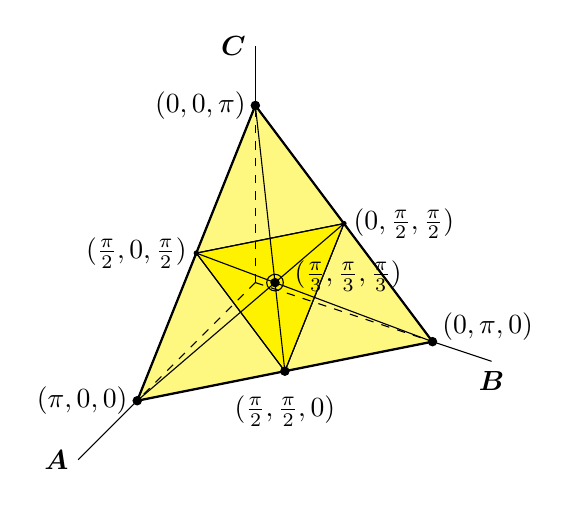
\begin{tikzpicture}[scale=.75]
		%Points
		\filldraw (0,3) circle (2pt); %top
		\filldraw (-2,-2) circle (2pt); %bottom left
		\filldraw (3,-1) circle (2pt); %bottom right
		\filldraw (1/3,0) circle (2pt); %centroid equilateral
		\draw (1/3,0) circle (4pt); %centroid equilateral
		\filldraw (1/2,-3/2) circle (2pt); %bottom midpoint
		\filldraw (-1,1/2) circle (1pt); %left midpoint
		\filldraw (3/2,1) circle (1pt); %right midpoint
		%\filldraw[orange] (-1/4,-1/2) circle (2pt); % right isosceles
		%\draw[orange] (-1/4,-1/2) circle (4pt);
		%Lines
		\draw[thick] (0,3)--(3,-1)--(-2,-2)--(0,3); %perimeter
		\draw (1/2,-3/2)--(-1,1/2)--(3/2,1)--(1/2,-3/2); %triangle of right triangles
		\draw[dashed] (0,0) -- (0,3); %z-axis
		\draw (0,3) -- (0,4); %z-axis end
		\draw[dashed] (0,0) -- (3,-1); %y-axis
		\draw (3,-1) -- (4,-4/3); %y-axis end
		\draw[dashed] (0,0) -- (-2,-2); %x-axis
		\draw (-2,-2) -- (-3,-3); %x-axis end
		\draw (0,3) -- (3,-1); %right side triangle
		\draw (0,3) -- (-2,-2); %left side triangle
		\draw (-2,-2) -- (3,-1); %bottom of triangle
		\draw (-2,-2) -- (3/2,1); %to midpoint on left side.
		\draw (0,3) -- (1/2,-3/2);
		\draw (3,-1) -- (-1,1/2);
		%\draw[ultra thick, red] (1/2,-3/2) -- (-1/4,-1/2);
		%\draw[ultra thick, blue] (-2,-2) -- (1/3,0);
		%\draw[ultra thick, blue] (1/2,-3/2) -- (1/3,0);
		%\draw[ultra thick, dashed, blue] (-2,-2) -- (1/2,-3/2);
		%Nodes
		\fill
		(0,3) node [left] {$(0,0,\pi)$}
		(3,-.75) node [right] {$(0,\pi,0)$}
		(-2,-2) node [left] {$(\pi,0,0)$}
		(1/2,-1.75) node [below] {$(\tfrac\pi 2,\tfrac\pi 2,0)$}
		(-1,1/2) node [left] {$(\tfrac\pi 2,0,\tfrac\pi 2)$}
		(3/2,1) node [right] {$(0,\tfrac\pi 2,\tfrac\pi 2)$}
		(9/18,1/9) node [right] {$(\tfrac{\pi}3,\tfrac{\pi}3,\tfrac{\pi}3)$};
		%(-1/3,-1/2) node [left] {$(\tfrac\pi 2,\tfrac\pi 4,\tfrac\pi 4)$};
		\node[left] at (-3,-3) {$\boldsymbol A$};
		\node[below] at (4,-4/3) {$\boldsymbol B$};
		\node[left] at (0,4) {$\boldsymbol C$};
		%shading
		\begin{scope}[on background layer]
		\draw[fill=yellow!50] (0,3)--(3,-1)--(-2,-2)--(0,3);
		%perimeter of obtuse restricted to x>y>z: (-2,-2) -- (1/2,-3/2) -- (-1/4,-1/2) -- (-2,-2);
		\draw[fill=yellow!100] (1/2,-3/2)--(-1,1/2)--(3/2,1)--(1/2,-3/2);
		%perimeter of acute restricted (1/3,0) -- (1/2,-3/2) -- (-1/4,-1/2) -- (1/3,0);
		\end{scope}
	\end{tikzpicture}
    \caption{The Triangle of Triangles $ \T$}
    \label{t-of-t}
\end{figure}
In Figure~\ref{t-of-t} the three altitudes represent isosceles triangles, 
and the darker inscribed triangular region represents the acute triangles.
The centroid is the equilateral triangle.
We refer to it as a moduli space, though technically it fails the universal
property, since the isosceles and equilateral points have nontrivial automorphisms.

\subsection{Using the Triangle of Triangles to Compute Things}\label{ComputeThings}
We like the representation of the space of triangles in Figure~\ref{t-of-t},
because it seems natural and is easy to analyze geometrically.
%\begin{figure}
%\centering
%\begin{tikzpicture}[scale=2]
%%Points
%\filldraw ({sqrt(3)/2},-1/2) circle (1pt); %bottom right
%\filldraw ({-sqrt(3)/2},-1/2) circle (1pt); %bottom left
%\filldraw (0,1) circle (1pt); %top
%\filldraw (0,0) circle (1pt); %centroid equilateral
%\draw (0,0) circle (2pt); %centroid
%\filldraw (0,-1/2) circle (.5pt); %bottom midpoint
%\filldraw ({-sqrt(3)/4},1/4) circle (.5pt);
%\filldraw ({sqrt(3)/4},1/4) circle (.5pt);
%%\filldraw[orange] (0,1/4) circle (.5pt); %right isosceles
%%\filldraw[orange] ({sqrt(3)/8},-1/8) circle (.5pt); %right isosceles
%%\filldraw[orange] ({-sqrt(3)/8},-1/8) circle (.5pt); %right isosceles
%%Lines
%\draw (0,1)--({-sqrt(3)/2},-1/2)--({sqrt(3)/2},-1/2)--(0,1); %outside triangle
%\draw (0,-1/2)--({sqrt(3)/4},1/4)--({-sqrt(3)/4},1/4)--(0,-1/2); %inside triangle
%\draw ({-sqrt(3)/2},-1/2)--({sqrt(3)/4},1/4);
%\draw ({sqrt(3)/2},-1/2)--({-sqrt(3)/4},1/4);
%\draw (0,1)--(0,-1/2);
%%shading
%\begin{scope}[on background layer]
%\draw[fill=yellow!100] (0,-1/2)--({sqrt(3)/4},1/4)--({-sqrt(3)/4},1/4)--(0,-1/2);
%\draw[fill=yellow!30] (0,1)--({-sqrt(3)/4},1/4)--({sqrt(3)/4},1/4)--(0,1); 
%\draw[fill=yellow!30] ({-sqrt(3)/4},1/4)--({-sqrt(3)/2},-1/2)--(0,-1/2)--({-sqrt(3)/4},1/4); 
%\draw[fill=yellow!30] ({sqrt(3)/4},1/4)--({sqrt(3)/2},-1/2)--(0,-1/2)--({sqrt(3)/4},1/4); 
%\end{scope}
%%nodes
%\node[below left] at ({-sqrt(3)/2},-1/2) {$(\pi,0,0)$};
%\node[below right] at ({sqrt(3)/2},-1/2) {$(0,\pi,0)$};
%\node[above left] at (0,1) {$(0,0,\pi)$};
%\end{tikzpicture}
%\caption{The Triangle of Triangles}
%\label{fig:t-of-t-simple}
%\end{figure}
It is certainly not original, see e.g. \cite[Figure 2]{ES15}.
With it we can compute things like dimension and relative measure.
It leads us to expect the acute and obtuse locus
to be two-dimensional, since those regions locally have two degrees of freedom.
It also suggests the loci of isosceles and right triangles should be one-dimensional,
which we know is true since one number is required to specify a right triangle or an isosceles triangle.
Additionally, the triangle of triangles predicts
\begin{enumerate}
\item
The ratio of obtuse to isosceles is $[3:1]$. This is because the triangle of acute triangles
is the (red) inscribed triangle, one of four equilateral triangles that partition the triangle of triangles.
\item
The ratio of obtuse-isosceles to acute-isosceles is $[1:1]$. This is because the altitudes 
represent isosceles triangles, and exactly half of each altitude lies in the triangle acute triangles.
\item
The ratio of isosceles to right triangles is $\left[2\cdot\tfrac{\sqrt 3}2:\tfrac 12\right]=2\sqrt 3$.
\end{enumerate}
Though this parameter space seems ``natural'' to us, there are other natural-seeming candidates, 
and, as mentioned above, they sometimes give different predictions for these numbers.
The reason is that in each one there is an implicit definition for the term ``random,'' 
and different constructions can differ in their implicit definitions.

\section{\bf The Torus of Triangles}

\subsection{Oriented Labeled Triangles}
Although we have just defined a triangle of triangles, we intend to replace it with something
more general. As mentioned above,
the question motivating this paper is, what happens when a continuous family of triangles in $\T^\circ$
crosses the border $\partial\T$?
The answer is that the triangles in the family change {\it orientation}.

An {\it orientation} of a labeled triangle is an assignment of a direction in which to traverse
the vertices. We say a triangle is {\it positively oriented} if the vertices are traversed counterclockwise,
and write $\tri ABC=(\alpha,\beta,\gamma)$;
otherwise we say it is {\it negatively oriented}, and write $-\tri ABC=(-\alpha,-\beta,-\gamma)$,
where $0\leq\alpha,\beta,\gamma\leq\pi$ in both cases.
Parameterize the negatively oriented elements
with $A+B+C=-\pi$ in the $(---)$-octant. As for the positively oriented elements,
this is a borderless triangle, which we denote by $-\T^\circ$. We call the closure
$-\T=-\T^\circ\sqcup-\partial\T$ the {\it shadow triangle of triangles}.

The border points $\partial\T$ and $-\partial\T$ are not, of course, proper triangles, 
since they are
triples with at least one zero entry; we say they are {\it degenerate} triangles.
Let $\LOTS=\T\sqcup-\T$ denote the set of labeled, oriented triangles up to similarity, including
the degenerate ones.
The two sets are illustrated in Figure \ref{fig:t-of-ts}.

\begin{figure}[h]
\centering
\begin{subfigure}{0.4\textwidth}
    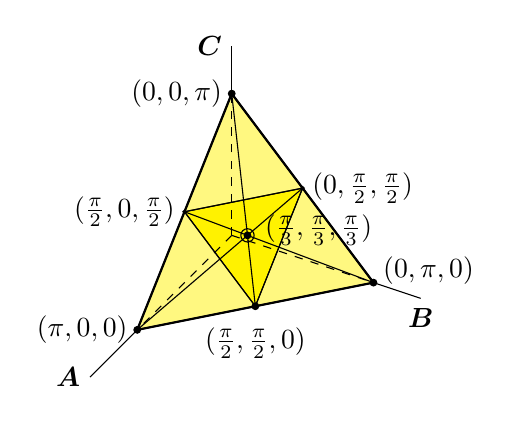
\begin{tikzpicture}[scale=.6]
		%Points
		\filldraw (0,3) circle (2pt); %top
		\filldraw (-2,-2) circle (2pt); %bottom left
		\filldraw (3,-1) circle (2pt); %bottom right
		\filldraw (1/3,0) circle (2pt); %centroid equilateral
		\draw (1/3,0) circle (4pt); %centroid equilateral
		\filldraw (1/2,-3/2) circle (2pt); %bottom midpoint
		\filldraw (-1,1/2) circle (1pt); %left midpoint
		\filldraw (3/2,1) circle (1pt); %right midpoint
		%\filldraw[orange] (-1/4,-1/2) circle (2pt); % right isosceles
		%\draw[orange] (-1/4,-1/2) circle (4pt);
		%Lines
		\draw[thick] (0,3)--(3,-1)--(-2,-2)--(0,3); %perimeter
		\draw (1/2,-3/2)--(-1,1/2)--(3/2,1)--(1/2,-3/2); %triangle of right triangles
		\draw[dashed] (0,0) -- (0,3); %z-axis
		\draw (0,3) -- (0,4); %z-axis end
		\draw[dashed] (0,0) -- (3,-1); %y-axis
		\draw (3,-1) -- (4,-4/3); %y-axis end
		\draw[dashed] (0,0) -- (-2,-2); %x-axis
		\draw (-2,-2) -- (-3,-3); %x-axis end
		\draw (0,3) -- (3,-1); %right side triangle
		\draw (0,3) -- (-2,-2); %left side triangle
		\draw (-2,-2) -- (3,-1); %bottom of triangle
		\draw (-2,-2) -- (3/2,1); %to midpoint on left side.
		\draw (0,3) -- (1/2,-3/2);
		\draw (3,-1) -- (-1,1/2);
		%\draw[ultra thick, red] (1/2,-3/2) -- (-1/4,-1/2);
		%\draw[ultra thick, blue] (-2,-2) -- (1/3,0);
		%\draw[ultra thick, blue] (1/2,-3/2) -- (1/3,0);
		%\draw[ultra thick, dashed, blue] (-2,-2) -- (1/2,-3/2);
		%Nodes
		\fill
		(0,3) node [left] {$(0,0,\pi)$}
		(3,-.75) node [right] {$(0,\pi,0)$}
		(-2,-2) node [left] {$(\pi,0,0)$}
		(1/2,-1.75) node [below] {$(\tfrac\pi 2,\tfrac\pi 2,0)$}
		(-1,1/2) node [left] {$(\tfrac\pi 2,0,\tfrac\pi 2)$}
		(3/2,1) node [right] {$(0,\tfrac\pi 2,\tfrac\pi 2)$}
		(9/18,1/9) node [right] {$(\tfrac{\pi}3,\tfrac{\pi}3,\tfrac{\pi}3)$};
		%(-1/3,-1/2) node [left] {$(\tfrac\pi 2,\tfrac\pi 4,\tfrac\pi 4)$};
		\node[left] at (-3,-3) {$\boldsymbol A$};
		\node[below] at (4,-4/3) {$\boldsymbol B$};
		\node[left] at (0,4) {$\boldsymbol C$};
		%shading
		\begin{scope}[on background layer]
		\draw[fill=yellow!50] (0,3)--(3,-1)--(-2,-2)--(0,3);
		%perimeter of obtuse restricted to x>y>z: (-2,-2) -- (1/2,-3/2) -- (-1/4,-1/2) -- (-2,-2);
		\draw[fill=yellow!100] (1/2,-3/2)--(-1,1/2)--(3/2,1)--(1/2,-3/2);
		%perimeter of acute restricted (1/3,0) -- (1/2,-3/2) -- (-1/4,-1/2) -- (1/3,0);
		\end{scope}
	\end{tikzpicture}
    \caption{Triangle of Triangles $ \T$}
    \label{fig:t-of-t}
\end{subfigure}
\hfill
\begin{subfigure}{0.5\textwidth}
    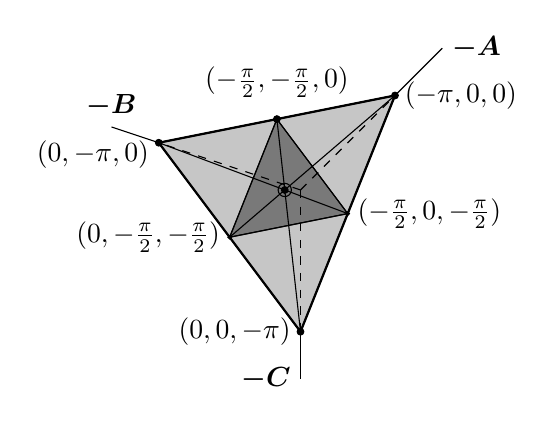
\begin{tikzpicture}[scale=.6]
	    \filldraw (10,-3) circle (2pt); %top
		\filldraw (12,2) circle (2pt); %bottom left
		\filldraw (7,1) circle (2pt); %bottom right
		\filldraw (10-1/3,0) circle (2pt); %centroid equilateral
		\draw (10-1/3,0) circle (4pt); %centroid equilateral
		\filldraw (10-1/2,3/2) circle (2pt); %bottom midpoint
		\filldraw (11,-1/2) circle (1pt); %left midpoint
		\filldraw (10-3/2,-1) circle (1pt); %right midpoint
		%Lines
		\draw[thick] (10,-3)--(7,1)--(12,2)--(10,-3); %perimeter
		\draw (10-1/2,3/2)--(11,-1/2)--(10-3/2,-1)--(10-1/2,3/2); %triangle of right triangles
		\draw[dashed] (10,0) -- (10,-3); %z-axis
		\draw (10,-3) -- (10,-4); %z-axis end
		\draw[dashed] (10,0) -- (7,1); %y-axis
		\draw (7,1) -- (6,4/3); %y-axis end
		\draw[dashed] (10,0) -- (12,2); %x-axis
		\draw (12,2) -- (13,3); %x-axis end
		\draw (10,-3) -- (7,1); %right side triangle
		\draw (10,-3) -- (12,2); %left side triangle
		\draw (12,2) -- (7,1); %bottom of triangle
		\draw (12,2) -- (10-3/2,-1); %to midpoint on left side.
		\draw (10,-3) -- (10-1/2,3/2);
		\draw (7,1) -- (11,-1/2);
		%Nodes
		\fill
		(10,-3) node [left] {$(0,0,-\pi)$}
		(7,.75) node [left] {$(0,-\pi,0)$}
		(12,2) node [right] {$(-\pi,0,0)$}
		(10-1/2,1.75) node [above] {$(-\tfrac\pi 2,-\tfrac\pi 2,0)$}
		(11,-1/2) node [right] {$(-\tfrac\pi 2,0,-\tfrac\pi 2)$}
		(10-3/2,-1) node [left] {$(0,-\tfrac\pi 2,-\tfrac\pi 2)$};
		\node[right] at (13,3) {$\boldsymbol{- A}$};
		\node[above] at (6,4/3) {$\boldsymbol {-B}$};
		\node[left] at (10,-4) {$\boldsymbol {-C}$};
		%shading
		\begin{scope}[on background layer]
		\draw[fill=darkgray!30] (10,-3)--(7,1)--(12,2)--(10,-3);
		\draw[fill=darkgray!70] (10-1/2,3/2)--(11,-1/2)--(10-3/2,-1)--(10-1/2,3/2);
		\end{scope}
	\end{tikzpicture}
    \caption{Shadow Triangle of Triangles $-\T$}
    \label{fig:shadow-t-of-t}
\end{subfigure}
\caption{\hspace{0cm}}
\label{fig:t-of-ts}
\end{figure}

\subsection{Main Theorem}

\begin{figure}[h]
\centering
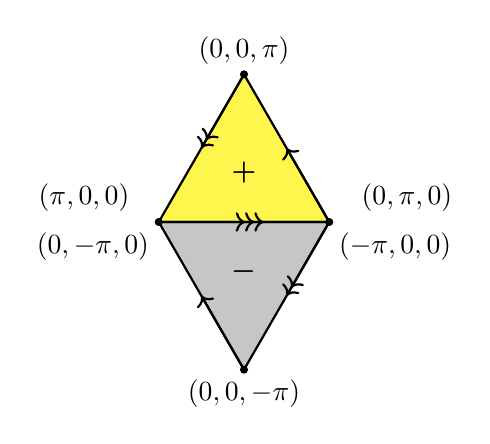
\begin{tikzpicture}[scale=2.5]
%Points
\filldraw (0,-1/4) circle (.5pt); %bottom
\filldraw ({-sqrt(3)/4},1/2) circle (.5pt); %left
\filldraw ({+sqrt(3)/4},1/2) circle (.5pt); %right
\filldraw (0,5/4) circle (.5pt); %top
%Lines
\draw[thick] (0,-1/4)--({+sqrt(3)/4},1/2)--({-sqrt(3)/4},1/2)--(0,-1/4); %bottom
\draw[thick] (0,5/4) --({+sqrt(3)/4},1/2)--({-sqrt(3)/4},1/2)--(0,5/4); %top
\draw[thick, ->] (0,-1/4)--({-sqrt(3)/8},1/8); %bottom
\draw[thick, ->>] ({+sqrt(3)/4},1/2)--({+sqrt(3)/8},1/8); %bottom
\draw[thick, ->>>] ({-sqrt(3)/4},1/2)--(.1,1/2); %middle
\draw[thick, ->] ({+sqrt(3)/4},1/2)--({+sqrt(3)/8},7/8);
\draw[thick, ->>] (0,5/4)--({-sqrt(3)/8},7/8); %bottom
%shading
\begin{scope}[on background layer]
\draw[fill=darkgray!30] (0,-1/4)--({+sqrt(3)/4},1/2)--({-sqrt(3)/4},1/2)--(0,-1/4);
\draw[fill=yellow!70] (0,5/4) --({+sqrt(3)/4},1/2)--({-sqrt(3)/4},1/2)--(0,5/4);
\end{scope}
%Nodes
\node[below] at (0,-1/4) {$(0,0,-\pi)$};
\node[left] at ({-.1-sqrt(3)/4},1/2+1/8) {$(\pi,0,0)$};
\node[right] at ({.115+sqrt(3)/4},1/2+1/8) {$(0,\pi,0)$};
\node at ({-.35-sqrt(3)/4},1/2) {\tiny $\Vvert$};
\node at ({.35+sqrt(3)/4},1/2) {\tiny $\Vvert$};
\node[left] at ({-sqrt(3)/4},1/2-1/8) {$(0,-\pi,0)$};
\node[right] at ({+sqrt(3)/4},1/2-1/8) {$(-\pi,0,0)$};
\node[above] at (0,5/4) {$(0,0,\pi)$};
\node at (0,1/4) {$\boldsymbol -$};
\node at (0,3/4) {$\boldsymbol +$};
\end{tikzpicture}
\caption{$(\T\sqcup-\T)/\text{\normalsize $\sim$}$}
\label{glued}
\end{figure}

\begin{Theorem}
$\LOTS$ is naturally a topological torus. Explicitly,
\[\LOTS\;=\;\frac{\T\sqcup-\T}{\vphantom{T}\text{\Large $\sim$}}\]
where the relation is on $\partial\T$ and $-\partial\T$, illustrated by arrows in Figure~\ref{glued}, 
and given explicitly by
by
\begin{align*}
(\alpha,\beta,0)\in\partial\T\;&\sim\; (\alpha-\pi,\beta-\pi,0)\in-\partial\T\quad\text{when $\gamma=0$}\\
(\alpha,0,\gamma)\in\partial\T\;&\sim\; (\alpha-\pi,0,\gamma-\pi)\in-\partial\T\quad\text{when $\beta=0$}\\
(0,\beta,\gamma)\in\partial\T\;&\sim\; (0,\beta-\pi,\gamma-\pi)\in-\partial\T\quad\text{when $\alpha=0$}
\end{align*}
\end{Theorem}

\begin{proof}
To prove it we induce a quotient on the disjoint union $\T\sqcup-\T$ via a bijection with
a transparently topologically connected alternative parameter space for 
labeled oriented triangles, one that uses
a triangle's {\it relative arguments}.
For any three points $A,B,C$ inscribed in a circle,
let $t_A=\arg(A)-\arg(C)$ and $t_B=\arg(B)-\arg(C)$, the ``relative arguments'' of the points $A,B,C$, where an argument
is traversed counterclockwise from a fixed ray (see Figure \ref{fig:relatives}).
\begin{figure}[!h]
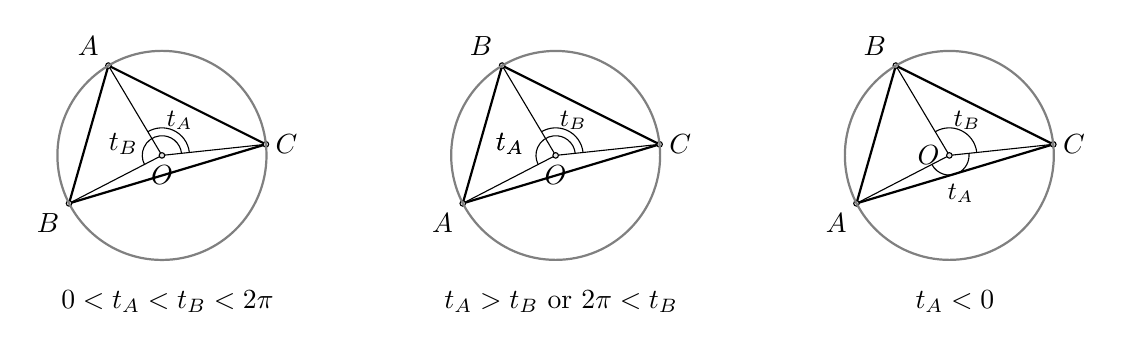
\begin{tikzpicture}
\tkzDefPoints{0/1/A,-.5/-.75/B,2/0/C}
\tkzDrawPolygon[thick](A,B,C)l
\tkzDefTriangleCenter[circum](A,B,C)
\tkzGetPoint{O}
\tkzMarkAngle[size=0.35](C,O,A)
\tkzLabelAngle[pos=0.5,font=\small](C,O,A){$t_A$}
\tkzMarkAngle[size=0.25](C,O,B)
\tkzDrawSegments[thin](O,A O,B O,C)
\tkzDrawPoints(A,B,C,O)
\tkzLabelPoints[above left](A)
\tkzLabelPoints[right](C)
\tkzLabelPoints[below left](B)
\tkzLabelPoints(O)
\tkzDefCircle[circum](A,B,C)
\tkzGetPoint{I}
\tkzDrawCircle[thick](I,A)
\node[left] at (.5,0) {$t_B$};
%%%%%
\tkzDefPoints{4.5/-.75/A, 5/1/B, 7/0/C} %added 5 to x.
\tkzDrawPolygon[thick](B,A,C)
\tkzDefTriangleCenter[circum](B,A,C)
\tkzGetPoint{O}
\tkzMarkAngle[size=0.25](C,O,A)
\tkzMarkAngle[size=0.35](C,O,B)
\tkzLabelAngle[pos=0.5,font=\small](C,O,B){$t_B$}
\tkzDrawSegments[thin](O,B O,A O,C)
\tkzDrawPoints(B,A,C,O)
\tkzLabelPoints[above left](B)
\tkzLabelPoints[right](C)
\tkzLabelPoints[below left](A)
\tkzLabelPoints(O)
\tkzDefCircle[circum](A,B,C)
\tkzGetPoint{I}
\tkzDrawCircle[thick](I,A)
\node[left] at (5.4,0) {$t_A$};
%%%%%
\tkzDefPoints{9.5/-.75/A, 10/1/B, 12/0/C} %added 10 to x.
\tkzDrawPolygon[thick](B,A,C)
\tkzDefTriangleCenter[circum](B,A,C)
\tkzGetPoint{O}
\tkzMarkAngle[size=0.25](A,O,C)
\tkzLabelAngle[pos=0.5,font=\small](A,O,C){$t_A$}
\tkzMarkAngle[size=0.35](C,O,B)
\tkzLabelAngle[pos=0.5,font=\small](C,O,B){$t_B$}
\tkzDrawSegments[thin](O,B O,A O,C)
\tkzDrawPoints(B,A,C,O)
\tkzLabelPoints[above left](B)
\tkzLabelPoints[right](C)
\tkzLabelPoints[below left](A)
\tkzLabelPoints[left](O)
\tkzDefCircle[circum](A,B,C)
\tkzGetPoint{I}
\tkzDrawCircle[thick](I,A)
\node[left] at (5.4,0) {$t_A$};
\node at (.75,-2) {$0<t_A < t_B<2\pi$};
\node at (5.75,-2) {$t_A>t_B$ or $2\pi<t_B$};
\node at (10.75,-2) {$t_A<0$};
\end{tikzpicture}
\caption{Relative Arguments}
\label{fig:relatives}
\end{figure}

Let $\mathsf R$ be the $t_A t_B$-plane.
It is clear that every pair of relative arguments defines a triangle, and that 
the triangle defined by a pair $(t_A,t_B)$ is positively oriented if and only if the representative
in the fundamental domain $0<t_A,t_B<2\pi$ satisfies $t_A<t_B$.
Thus
$\mathsf R$ is partitioned into triangles corresponding to positively
and negatively oriented triangles, shown in yellow and gray in Figure~\ref{fig:region-r}.

\begin{figure}
\centering
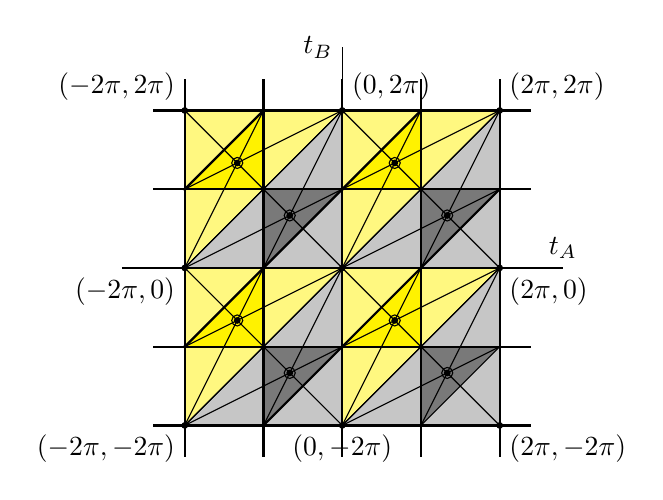
\begin{tikzpicture}%[scale=1.25]
%Points
\filldraw (0,0) circle (1pt);
\filldraw (0,2) circle (1pt); %mid left
\filldraw (2,2) circle (1pt); %mid right
\filldraw (2,0) circle (1pt); %lower right
\filldraw (-2,0) circle (1pt); %lower left
\filldraw (2,4) circle (1pt); %upper right
\filldraw (1,1) circle (.5pt); %isosceles point in Q_C
\filldraw (1,2) circle (.5pt); %isosceles point in Q_C
\filldraw (0,1) circle (.5pt); %isosceles point in Q_C
\filldraw (2,3) circle (.5pt);%isosceles in Q_B
\filldraw (1,3) circle (.5pt); %isosceles in Q_B
\filldraw (-1,0) circle (.5pt); %isosceles in Q_A
\filldraw (-1,1) circle (.5pt); %isosceles in Q_A
\filldraw (0,4) circle (.5pt); %top point on t_B axis.
\filldraw (2/3,4/3) circle (1pt); %equilateral in T
\draw (2/3,4/3) circle (2pt); %equilateral in T
\filldraw (4/3,2/3) circle (1pt); %equilateral in Q_C
\draw (4/3,2/3) circle (2pt); %equilateral in Q_C
\filldraw (4/3,2/3+2) circle (1pt); %equilateral in Q_A
\draw (4/3,2/3+2) circle (2pt); %equilateral in Q_A
\filldraw (4/3-2,2/3) circle (1pt); %equilateral in Q_B
\draw (4/3-2,2/3) circle (2pt); %equilateral in Q_B
% adding upper left part
\filldraw (-2,2) circle (1pt);
\filldraw (-2,4) circle (1pt);
\filldraw (0,4) circle (1pt);
\filldraw (-2,1) circle (.5pt);
\filldraw (-2,3) circle (.5pt);
\filldraw (-1,2) circle (.5pt);
\filldraw (-1,3) circle (.5pt);
\filldraw (-1,4) circle (.5pt);
\filldraw (0,3) circle (.5pt);
\filldraw (0,4) circle (.5pt);
\filldraw (1,4) circle (.5pt);
\filldraw (-1-1/3,4/3) circle (1pt); %equilateral in lower left yellow
\draw (-1-1/3,4/3) circle (2pt); %equilateral in lower left yellow
\filldraw (-1-1/3,3+1/3) circle (1pt); %equilateral in upper left yellow
\draw (-1-1/3,3+1/3) circle (2pt); %equilateral in upper left yellow
\filldraw (2/3,1/3+3) circle (1pt); %equilateral in upper right yellow
\draw (2/3,1/3+3) circle (2pt); %equilateral in upper right yellow
\filldraw (-2/3,2+2/3) circle (1pt); %equilateral in upper left gray
\draw (-2/3,2+2/3) circle (2pt); %equilateral in upper left gray

%Lines
\draw (0,2)--(0,4.5); %y-axis.
\draw (0,2)--(2.5,2); %x-axis.
\draw[] (0,0)--(0,2)--(2,2)--(2,0)--(0,0); %perimeter of OG pic
\draw[] (0,0)--(2,2); %diagonal of OG pic
\draw[] (-2,2)--(0,4); %diagonal of upper left pic
\draw[] (-2,0)--(2,4)--(2,0)--(-2,0); %perimater of T#
\draw[] (-2,0)--(-2,4)--(2,4); %perimeter of upper half
\draw[] (-2,2)--(0,2)--(0,4); %perimeter of upper left square
%\draw (0,1)--(1,1)--(1,2)--(0,1); %dark yellow triangle
%\draw (1,0)--(1,1)--(2,1)--(1,0); %black triangle
\draw[thick,black] (-2.4,0)--(2.4,0); %horizontal
\draw[thick,black] (-2.4,1)--(2.4,1); %horizontal
\draw[thick,black] (-2.4,2)--(2.4,2); %horizontal
\draw[black] (-2.8,2)--(2.8,2); %horizontal axis
\draw[thick,black] (-2.4,3)--(2.4,3); %horizontal
\draw[thick,black] (-2.4,4)--(2.4,4); %horizontal
\draw[thick,black] (-2,-.4)--(-2,4.4); %vertical
\draw[thick,black] (-1,-.4)--(-1,4.4); %vertical
\draw[thick,black] (0,-.4)--(0,4.4); %vertical
\draw[black] (0,0)--(0,4.8); %vertical axis
\draw[thick,black] (1,-.4)--(1,4.4); %vertical
\draw[thick,black] (2,-.4)--(2,4.4); %vertical
\draw[thick,black] (-1,0)--(2,3); %diagonal
\draw[thick,black] (-2,1)--(1,4); %diagonal
\draw[thick,black] (-2,3)--(-1,4); %diagonal
\draw (0,0)--(2,1); %shallow isosceles
\draw (-2,0)--(2,2); %shallow isosceles
\draw (-2,1)--(2,3); %shallow isosceles
\draw (-2,2)--(2,4); %shallow isosceles
\draw (-2,3)--(0,4); %shallow isosceles
\draw (1,0)--(2,2); %steep isosceles
\draw (0,0)--(2,4); %steep isosceles
\draw (-1,0)--(1,4); %steep isosceles
\draw (-2,0)--(0,4); %steep isosceles
\draw (-2,2)--(-1,4); %steep isosceles
\draw (-2,2)--(0,0); %negative isosceles
\draw (-2,4)--(2,0); %negative isosceles
\draw (0,4)--(2,2); %negative isosceles

%Colors
\begin{scope}[on background layer]
\draw[fill=darkgray!30] (0,0)--(2,2)--(2,0)--(0,0); %lower right
\draw[fill=darkgray!30] (2,2)--(2,4)--(0,2)--(2,2); %upper right
\draw[fill=darkgray!30] (-2,0)--(0,0)--(0,2)--(-2,0); %upper right
\draw[fill=yellow!50] (0,0)--(0,2)--(2,2)--(0,0);
\draw[fill=yellow!100] (1,1)--(1,2)--(0,1)--(1,1);
\draw[fill=darkgray!70] (1,0)--(1,1)--(2,1)--(1,0); %lower right acute
\draw[fill=darkgray!70] (1,2)--(1,3)--(2,3)--(1,2); %lower left acute
\draw[fill=darkgray!70] (-1,0)--(-1,1)--(0,1)--(-1,0); %above right acute
% upper left half
\draw[fill=yellow!50] (-2,0)--(-2,2)--(0,2)--(-2,0); % lower left yellow
\draw[fill=yellow!100] (-2,1)--(-1,2)--(-1,1)--(-2,1); %lower left yellow acute
\draw[fill=yellow!50] (-2,2)--(-2,4)--(0,4)--(-2,2); % upper left yellow
\draw[fill=yellow!100] (-2,3)--(-1,4)--(-1,3)--(-2,3); %upper left yellow acute
\draw[fill=yellow!50] (0,2)--(0,4)--(2,4)--(0,2); % upper right yellow
\draw[fill=yellow!100] (0,3)--(1,4)--(1,3)--(0,3); %upper right yellow acute
\draw[fill=darkgray!30] (-2,2)--(0,4)--(0,2)--(-2,2); % upper left gray
\draw[fill=darkgray!70] (-1,2)--(-1,3)--(0,3)--(-1,2); %upper left gray acute


\end{scope}
%Nodes
%\node[left] at (0,2) {$(0,2\pi)$};
\node[below right] at (2,0) {$(2\pi,-2\pi)$};
\node[above right] at (0,4) {$(0,2\pi)$};
\node[above right] at (2,4) {$(2\pi,2\pi)$};
\node[below left] at (-2,0) {$(-2\pi,-2\pi)$};
\node[below] at (0,0) {$(0,-2\pi)$};
\node[below left] at (-2,2) {$(-2\pi,0)$};
\node[above left] at (-2,4) {$(-2\pi,2\pi)$};
\node[below right] at (2,2) {$(2\pi,0)$};
\node[above right] at (2.5,2) {$t_A$};
\node[left] at (0,4.8) {$t_B$};
\end{tikzpicture}
\caption{The Plane $\mathsf R$}
\label{fig:region-r}
\end{figure}
It is also clear that 
points in $\mathsf R$ determine the same triangle if and only if they are congruent $\pmod{2\pi}$.
Since every triangle has a set of relative arguments,
the assignment of $\tri ABC$ to a point $(t_A,t_B)$ defines a surjective map
\[\tri\;:\;\mathsf R\longrightarrow\LOTS\]
that induces a bijection $\mathsf R/2\pi\isim\LOTS$, realizing
$\LOTS$ as the topological torus of Figure~\ref{fig:R/2pi}.
\begin{figure}[h]
%\centering
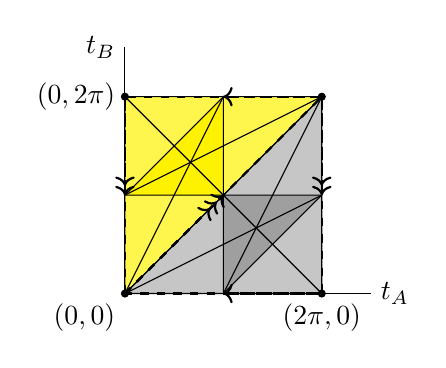
\begin{tikzpicture}
[scale=1.25]
%Points
\filldraw (0,0) circle (1pt); %mid bottom
\filldraw (0,2) circle (1pt); %top left
\filldraw (2,2) circle (1pt); %top right
\filldraw (2,0) circle (1pt); %botom right
%\filldraw (1,1) circle (.5pt); %isosceles point in Q_C
%\filldraw (1,2) circle (.5pt); %isosceles point in Q_C
%\filldraw (0,1) circle (.5pt); %isosceles point in Q_C
%Lines
\draw[thick, dashed] (0,0)--(0,2)--(2,2)--(2,0)--(0,0); %perimeter
\draw[thick, dashed] (0,0)--(2,2); %diagonal
\draw (0,0)--(0,2.5); %y-axis.
\draw (0,0)--(2.5,0); %x-axis.
\draw[thick, dashed, ->] (2,2)--(1,2);
\draw[thick, dashed, ->] (2,0)--(1,0);
\draw[thick, dashed, ->>] (0,2)--(0,1);
\draw[thick, dashed, ->>] (2,2)--(2,1);
\draw[thick, dashed, ->>>] (0,0)--(1,1);
\draw[thin] (0,2)--(2,0); %thin isosceles line
\draw[thin] (0,1)--(2,2); %thin isosceles line
\draw[thin] (0,0)--(1,2); %thin isosceles line
\draw[thin] (0,0)--(2,1);
\draw[thin] (1,0)--(2,2);
%Colors
\begin{scope}[on background layer]
\draw[fill=darkgray!30] (0,0)--(2,2)--(2,0)--(0,0); %lower right
\draw[fill=yellow!70] (0,0)--(2,2)--(0,2)--(0,0); %yellow perimeter
\draw[thin, fill=yellow!100] (1,1)--(1,2)--(0,1)--(1,1); %yellow acute
\draw[thin, fill=darkgray!50] (1,0)--(1,1)--(2,1)--(1,0); %lower right acute
\end{scope}
%Nodes
\node[left] at (0,2) {$(0,2\pi)$};
\node[below] at (2,0) {$(2\pi,0)$};
\node[below left] at (0,0) {$(0,0)$};
\node[right] at (2.5,0) {$t_A$};
\node[left] at (0,2.5) {$t_B$};
\end{tikzpicture}
\caption{$\mathsf R/2\pi$ is a Torus} 
\label{fig:R/2pi}
\end{figure}

To compute $\tri$, which takes a pair of relative arguments to a triple
of angles, either on $\T$ or $-\T$, we use Euclid III.20 
\cite[III Proposition 20]{Euclid},
which states,
{\it in a circle the angle at the center is double the angle at 
the circumference, when the angles have the same circumference as base.}
Let $[t_A]$ and $[t_B]$ denote representatives of $t_A\pmod{2\pi}$ and $t_B\pmod{2\pi}$
in the interval $[0,2\pi]$, where the choice of $0$ or $2\pi$ will be clear from context. 
Applying Euclid III.20 to Figure~\ref{fig:relatives} yields
\[\tri(t_A,t_B)=\begin{cases}
\left(\frac 12(2\pi-[t_B]),\,\frac 12 [t_A],\,\frac 12([t_B]-[t_A])\right)\in\T&\text{if $0<[t_A]< [t_B]<2\pi$}\\[2pt]
\left(-\frac 12[t_B],\,-\frac 12(2\pi-[t_A]),\,\frac 12([t_B]-[t_A])\right)\in-\T&\text{if $0<[t_B]< [t_A]<2\pi$}\\
\end{cases}
\]
Thus $\tri$ maps the yellow regions to positively oriented triangles in $\T^\circ$, and the gray
regions to negatively oriented triangles, in $-\T^\circ$.
The triangle $\tri(t_A,t_B)$ is degenerate if $[t_B]-[t_A], [t_A]$, or $[t_B]$ is $0$,
in which cases two vertices coincide.
In these cases the formula for $\tri(t_A,t_B)$ identifies points on
the borders as follows:
\[
\begin{cases}
\left(\pi-\frac 12[t_A],\,\frac 12 [t_A],\,0\right)\in\T
\longleftrightarrow
\left(-\frac 12[t_A],\,-\pi+\frac 12[t_A],\,0\right)\in-\T
&\text{if $[t_B]-[t_A]=0$}\\[2pt]
\left(\pi-\frac 12[t_B],\,0,\,\frac 12[t_B]\right)\in\T
\longleftrightarrow
\left(-\frac 12[t_B],\,0,\,-\pi+\frac 12[t_B]\right)\in-\T
&\text{if $t_A\equiv 0\equiv 2\pi$}\\[2pt]
\left(0,\,\frac 12 [t_A],\,\pi-\frac 12[t_A]\right)\in\T
\longleftrightarrow
\left(0,\,-\pi+\frac 12[t_A],\,-\frac 12[t_A]\right)\in-\T
&\text{if $t_B\equiv 2\pi\equiv 0$}
\end{cases}\]
%Note the border of $\T$ is at $t_A=0$ and $t_B=2\pi$,
%whereas the border of $-\T$ is at $t_A=2\pi$ and $t_B=0$.
This matches the statement of the theorem, and completes the proof.
\end{proof}

\begin{figure}[h]
	\centering
	\includegraphics[width=0.4\textwidth]{pics/torus-right-isosceles-degenerate.png}
	\caption{The Torus of Triangles}
	\label{fig:torus-of-t}
\end{figure}

The torus of triangles is drawn
in Figure \ref{fig:torus-of-t}.
The yellow and gray regions represent the positively- 
and negatively-oriented triangles. The red curves at 
the boundaries of the positively- and negatively-oriented regions are degenerate triangles. 
The blue and black curves are the isosceles and right families, respectively. 
The triple intersection point of the blue isosceles curves in the yellow region 
is the positively-oriented equilateral triangle point; this point has a negatively-oriented counterpart
in the gray region. 
The point shown on the front of the torus in Figure \ref{fig:torus-of-t}, 
where the three red and three blue curves intersect, corresponds to the identified
four corners of the fundamental polygon.

\begin{Remark}
The linear map taking the $t_A t_B$-plane $\mathsf R$ to the plane $A+B+C=\pi$ on which
we find $\T$ is 
\[(\pi,0,0)\;+\;\bmxr{0&-\frac 12\\[2pt]\frac 12&0\\[2pt]-\frac 12&\frac 12}\]
with area distortion factor $\frac{\sqrt 3}4$. Since lengths are
distorted nonuniformly,
the fundamental domain $\mathsf R/2\pi$
computes the same information about different types of triangles with respect to area,
but not with respect to length, as 
the original moduli space $\T$ in Subsection~\ref{ComputeThings}.
\end{Remark}



\section{\bf Examples of Families}
\label{sec:examples}

A torus has a nontrivial fundamental group, and therefore contains ``nontrivial'' loops, loops not contractible
to a point. 
The families of degenerate, isosceles, and right (oriented labeled) triangles all
determine nontrivial loops. 

\subsection{A Trivial Family}
Several concentric trivial loops of triangles are shown in purple on the torus in Figure \ref{fig:torus-trivial}, 
and in the $(t_A,t_B)$-plane in Figure \ref{fig:plane-trivial}. 
These families form circles in the plane, all contractible to a point. 
The actual (3-sided) triangles in one of these families are illustrated in Figure~\ref{fig:trivial-pencil}. 

\begin{figure}[h]
\centering
\begin{subfigure}{0.4\textwidth}
	\centering
     \includegraphics[width=0.75\textwidth]{pics/torus-trivial-family-nontrivial-loop.png}
	\caption{On the Torus.}
	\label{fig:torus-trivial}
\end{subfigure}
%\hfill
\begin{subfigure}{0.55\textwidth}
	\centering
    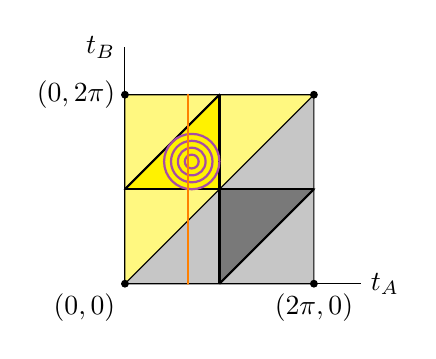
\begin{tikzpicture}[scale=1.2]
%Points
\filldraw (0,0) circle (1pt);
\filldraw (0,2) circle (1pt); %mid left
\filldraw (2,2) circle (1pt); %mid right
\filldraw (2,0) circle (1pt); %lower right
%\filldraw (1,1) circle (.5pt); %isosceles point in Q_C
%\filldraw (1,2) circle (.5pt); %isosceles point in Q_C
%\filldraw (0,1) circle (.5pt); %isosceles point in Q_C
%\filldraw (2/3,4/3) circle (1pt); %equilateral in T
%\draw (2/3,4/3) circle (2pt); %equilateral in T
%\filldraw (4/3,2/3) circle (1pt); %equilateral in Q_C
%\draw (4/3,2/3) circle (2pt); %equilateral in Q_C

\draw (0,0)--(0,2.5); %y-axis.
\draw (0,0)--(2.5,0); %x-axis.

%Lines
%\draw[thick, red] (0,0)--(0,2)--(2,2)--(2,0)--(0,0); %perimeter of OG pic
%\draw[thick, red] (0,0)--(2,2); %diagonal of OG pic
%\draw[thick, dashed] (-2,0)--(2,4)--(2,0)--(-2,0); %perimater of T#
\draw (0,1)--(1,1)--(1,2)--(0,1); %dark yellow triangle
\draw (1,0)--(1,1)--(2,1)--(1,0); %black triangle
% RIGHT
\draw [thick,black] (0,1)--(2,1); %horizontal
\draw [thick,black] (1,0)--(1,2); %vertical
\draw [thick,black] (0,1)--(1,2); %diagonal
\draw [thick,black] (1,0)--(2,1); %diagonal
%ISOSCELES
%\draw [thick, blue](0,2)--(2,0);
%\draw [thick, blue](0,1)--(2,2);
%\draw [thick, blue](0,0)--(2,1);
%\draw [thick, blue](0,0)--(1,2);
%\draw [thick, blue](1,0)--(2,2);


%Colors
\begin{scope}[on background layer]
\draw[fill=darkgray!30] (0,0)--(2,2)--(2,0)--(0,0); %lower right


\draw[fill=yellow!100] (1,1)--(1,2)--(0,1)--(1,1);
\draw[fill=yellow!50] (1,1)--(1,2)--(2,2)--(1,1);
\draw[fill=yellow!50] (1,1)--(0,0)--(0,1)--(1,1);
\draw[fill=yellow!50] (0,1)--(0,2)--(1,2)--(0,1);
\draw[fill=darkgray!70] (1,0)--(1,1)--(2,1)--(1,0); %lower right acute

\end{scope}
%Nodes
\node[left] at (0,2) {$(0,2\pi)$};
\node[below] at (2,0) {$(2\pi,0)$};
\node[below left] at (0,0) {$(0,0)$};
\node[right] at (2.5,0) {$t_A$};
\node[left] at (0,2.5) {$t_B$};
%\node at (0,-.5) {The region $\mathsf R$};
% trivial family circle
\tkzDefPoint(sqrt(2)/2,2-sqrt(2)/2){I}
\tkzDefPoint(1,2-sqrt(2)/2){I_1} %largest , 100% radius
\tkzDefPoint(sqrt(2)/8+3/4,2-sqrt(2)/2){I_2} %75% radius
\tkzDefPoint(sqrt(2)/4+1/2,2-sqrt(2)/2){I_3} %50% radius
\tkzDefPoint(3*sqrt(2)/8+1/4,2-sqrt(2)/2){I_4} %25% radius
\tkzDrawCircles[thick,violet!70!white](I,I_1 I,I_2 I,I_3 I,I_4)
% orange line
\tkzDefPoint(2/3,0){Y}
\tkzDefPoint(2/3,2){Z}
\tkzDrawSegment[thick,orange](Y,Z)

\end{tikzpicture}
\caption{In $\mathsf R/2\pi$}
\label{fig:plane-trivial}
\end{subfigure}       
\caption{Trivial Families and a Nontrivial Family}
\label{fig:trivial-family}
\end{figure}

\begin{figure}
\centering
\begin{subfigure}{0.45\textwidth}
\centering
\definecolorseries{first}{rgb}{last}{red}{yellow}
\definecolorseries{second}{rgb}{last}{yellow}{blue}
\definecolorseries{third}{rgb}{last}{blue}{red}
\begin{tikzpicture}[scale=0.75]
	    \def\outRadius{2} % outcircle
	    \def\penRadius{0.75*pi*(1-sqrt(2)/2)} % circle in t_A,t_B plane
	    \def\xA{pi*(sqrt(2)/2)}
	    \def\yA{pi*(2-(sqrt(2)/2))}
	    \tkzDefPoint(0,0){O}
	    \tkzDefPoint(0:\outRadius){C}
	    
	    \resetcolorseries[15]{first}
	    \foreach \t in {0,0.05,...,0.65}{
	    	\tkzDefPoint(\outRadius*cos(\penRadius*cos(\t*pi)+\xA),\outRadius*sin(\penRadius*cos(\t*pi)+\xA)){A}
	    	\tkzDefPoint(\outRadius*cos(\penRadius*sin(\t*pi)+\yA),\outRadius*sin(\penRadius*sin(\t*pi)+\yA)){B}
	     \draw [very thick,color=first!!+](A) -- (B) -- (C) -- (A);
		}
		\resetcolorseries[15]{second}
        \foreach \t in {0.65,0.7,...,1.35}{
	    	\tkzDefPoint(\outRadius*cos(\penRadius*cos(\t*pi)+\xA),\outRadius*sin(\penRadius*cos(\t*pi)+\xA)){A}
	    	\tkzDefPoint(\outRadius*cos(\penRadius*sin(\t*pi)+\yA),\outRadius*sin(\penRadius*sin(\t*pi)+\yA)){B}
	     \draw [very thick,color=second!!+](A) -- (B) -- (C) -- (A);
		}
		\resetcolorseries[15]{third}
        \foreach \t in {1.35,1.4,...,2}{
	    	\tkzDefPoint(\outRadius*cos(\penRadius*cos(\t*pi)+\xA),\outRadius*sin(\penRadius*cos(\t*pi)+\xA)){A}
	    	\tkzDefPoint(\outRadius*cos(\penRadius*sin(\t*pi)+\yA),\outRadius*sin(\penRadius*sin(\t*pi)+\yA)){B}
	     \draw [very thick,color=third!!+](A) -- (B) -- (C) -- (A);
		}
		% special triangle
		\def\arg{0.75} %make sure to change for other figure as well
		\tkzDefPoint(\outRadius*cos(\penRadius*cos(\arg*pi)+\xA),\outRadius*sin(\penRadius*cos(\arg*pi)+\xA)){A}
	    \tkzDefPoint(\outRadius*cos(\penRadius*sin(\arg*pi)+\yA),\outRadius*sin(\penRadius*sin(\arg*pi)+\yA)){B}
	    \draw [ultra thick,black](A) -- (B) -- (C) -- (A);
	    \tkzDrawCircle[very thick, black](O,C)
	    \tkzDrawPoints[ultra thick, black](A,B,C)
	    \tkzLabelPoint[above](A){$A(t_A)$}
	    \tkzLabelPoint[below](B){$B(t_B)$}
	    \tkzLabelPoint[right](C){$C$}
\end{tikzpicture}
\caption{The Family Inscribed in a Circle.}
\label{fig:trivial-pencil}
\end{subfigure}
%\hfill
\begin{subfigure}{0.45\textwidth}
\centering
\begin{tikzpicture}[scale=1.2]
\begin{scope}[on background layer]
\draw[fill=darkgray!30] (0,0)--(2,2)--(2,0)--(0,0); %lower right


\draw[fill=yellow!70] (1,1)--(1,2)--(0,1)--(1,1);
\draw[fill=yellow!30] (1,1)--(1,2)--(2,2)--(1,1);
\draw[fill=yellow!30] (1,1)--(0,0)--(0,1)--(1,1);
\draw[fill=yellow!30] (0,1)--(0,2)--(1,2)--(0,1);
\draw[fill=darkgray!70] (1,0)--(1,1)--(2,1)--(1,0); %lower right acute
 \end{scope}
%Points
\filldraw (0,0) circle (1pt);
\filldraw (0,2) circle (1pt); %mid left
\filldraw (2,2) circle (1pt); %mid right
\filldraw (2,0) circle (1pt); %lower right
\filldraw (1,1) circle (.5pt); %isosceles point in Q_C
\filldraw (1,2) circle (.5pt); %isosceles point in Q_C
\filldraw (0,1) circle (.5pt); %isosceles point in Q_C
% \filldraw (2/3,4/3) circle (1pt); %equilateral in T
% \draw (2/3,4/3) circle (2pt); %equilateral in T
% \filldraw (4/3,2/3) circle (1pt); %equilateral in Q_C
% \draw (4/3,2/3) circle (2pt); %equilateral in Q_C


\draw (0,0)--(0,2.5); %y-axis.
\draw (0,0)--(2.5,0); %x-axis.

%Lines
%\draw[red,thick] (0,0)--(0,2)--(2,2)--(2,0)--(0,0); %perimeter of OG pic
%\draw[red,thick] (0,0)--(2,2); %diagonal of OG pic
%\draw[thick, dashed] (-2,0)--(2,4)--(2,0)--(-2,0); %perimater of T#
\draw (0,1)--(1,1)--(1,2)--(0,1); %dark yellow triangle
\draw (1,0)--(1,1)--(2,1)--(1,0); %black triangle
% RIGHT
\draw [black] (0,1)--(2,1); %horizontal
\draw [black] (1,0)--(1,2); %vertical
\draw [black] (0,1)--(1,2); %diagonal
\draw [black] (1,0)--(2,1); %diagonal
%ISOSCELES
\draw [black](0,2)--(2,0);
\draw [black](0,1)--(2,2);
\draw [black](0,0)--(2,1);
\draw [black](0,0)--(1,2);
\draw [black](1,0)--(2,2);


%Colors

%Nodes
\node[left] at (0,2) {$(0,2\pi)$};
\node[below] at (2,0) {$(2\pi,0)$};
\node[below left] at (0,0) {$(0,0)$};
\node[right] at (2.5,0) {$t_A$};
\node[left] at (0,2.5) {$t_B$};
%\node at (0,-.5) {The region $\mathsf R$};
% trivial family circle
\tkzDefPoint(sqrt(2)/2,2-sqrt(2)/2){I}
\tkzDefPoint(1,2-sqrt(2)/2){I_1} %largest , 100% radius
% \tkzDefPoint(sqrt(2)/8+3/4,2-sqrt(2)/2){I_2} %75% radius
% \tkzDefPoint(sqrt(2)/4+1/2,2-sqrt(2)/2){I_3} %50% radius
% \tkzDefPoint(3*sqrt(2)/8+1/4,2-sqrt(2)/2){I_4} %25% radius
% rainbow circle
\tkzCalcLength(I,I_1)\tkzGetLength{radius}
\resetcolorseries[360]{first}
\foreach \t in {0,0.01,...,0.7}{
    \tkzDefPoint(0.75*(1-(sqrt(2)/2))*cos(\t*pi)+(sqrt(2)/2),0.75*(1-(sqrt(2)/2))*sin(\t*pi)+(2-sqrt(2)/2)){P}
    \tkzDrawPoint[thin, color=first!!+](P)
}
\resetcolorseries[330]{second}
\foreach \t in {0.71,0.72,...,1.35}{
    \tkzDefPoint(0.75*(1-(sqrt(2)/2))*cos(\t*pi)+(sqrt(2)/2),0.75*(1-(sqrt(2)/2))*sin(\t*pi)+(2-sqrt(2)/2)){P}
    \tkzDrawPoint[thin, color=second!!+](P)
}
\resetcolorseries[330]{third}
\foreach \t in {1.36,1.37,...,2}{
    \tkzDefPoint(0.75*(1-(sqrt(2)/2))*cos(\t*pi)+(sqrt(2)/2),0.75*(1-(sqrt(2)/2))*sin(\t*pi)+(2-sqrt(2)/2)){P}
    \tkzDrawPoint[thin, color=third!!+](P)
}
% special black dot
\def\arg{0.75}
\tkzDefPoint(0.75*(1-(sqrt(2)/2))*cos(\arg*pi)+(sqrt(2)/2),0.75*(1-(sqrt(2)/2))*sin(\arg*pi)+(2-sqrt(2)/2)){T}
\tkzDrawPoint[black, thick](T)
\tkzLabelPoint[left](T){$\triangle{ABC}$}

\end{tikzpicture}
\caption{The Family in $\mathsf R/2\pi$}
\label{fig:trivial-key}
\end{subfigure}
\caption{The Triangles in a Trivial Family. Point $\triangle{ABC}$ in Figure \ref{fig:trivial-key} represents $\triangle{ABC}$ in Figure \ref{fig:trivial-pencil}.}
\label{fig:trivial}
\end{figure}

\subsection{A Nontrivial Family}
A nontrivial family of actual (3-sided) triangles is illustrated in Figures \ref{fig:nontrivial-pencil} and \ref{fig:torus-trivial}. 
This family is generated by fixing vertices $A$ and $C$ and allowing $B$ to wander around the circle. 
Notice how the warm-colored triangles are negatively-oriented and thus located in the gray triangle, 
while the cool-colored triangles are positively-oriented and located in the yellow triangle. 
The yellow triangles in Figure \ref{fig:nontrivial-pencil} are almost degenerate triangles, 
which is seen in Figure \ref{fig:nontrivial-key} 
by the yellow color of the gradient when it cross the diagonal line, which represents degenerate triangles. 


\begin{figure}
\centering
\begin{subfigure}{0.45\textwidth}
\centering
\definecolorseries{first}{rgb}{last}{red}{yellow}
\definecolorseries{second}{rgb}{last}{yellow}{blue}
\definecolorseries{third}{rgb}{last}{blue}{red}
\begin{tikzpicture}[scale=0.75]
	    \def\outRadius{2} % outcircle
	    \tkzDefPoint(0,0){O}
	    \tkzDefPoint(0:\outRadius){C}
	    \tkzDefPoint(120: \outRadius){A}
	    \resetcolorseries[13]{first}
	    \foreach \t in {0,10,...,120}{
	    	\tkzDefPoint(\t:\outRadius){B}
	     \draw [very thick,color=first!!+](A) -- (B) -- (C) -- (A);
		}
 		\resetcolorseries[13]{second}
        \foreach \t in {120,130,...,240}{
	    	\tkzDefPoint(\t:\outRadius){B}
	     \draw [very thick,color=second!!+](A) -- (B) -- (C) -- (A);
		}
 		\resetcolorseries[13]{third}
        \foreach \t in {250,260,...,350}{
	    	\tkzDefPoint(\t:\outRadius){B}
	     \draw [very thick,color=third!!+](A) -- (B) -- (C) -- (A);
		}
		% special triangle
		\def\arg{240} %make sure to change for other figure as well
	    \tkzDefPoint(\arg:\outRadius){B}
	    \draw [ultra thick,black](A) -- (B) -- (C) -- (A);
	    \tkzDrawCircle[very thick, black](O,C)
	    \tkzDrawPoints[ultra thick, black](A,B,C)
	    \tkzLabelPoint[above](A){$A$}
	    \tkzLabelPoint[below](B){$B(t_B)$}
	    \tkzLabelPoint[right](C){$C$}
\end{tikzpicture}
\caption{The Family Inscribed in a Circle.}
\label{fig:nontrivial-pencil}
\end{subfigure}
\hfill
\begin{subfigure}{0.45\textwidth}
\centering
\begin{tikzpicture}[scale=1.2]
\begin{scope}[on background layer]
\draw[fill=darkgray!30] (0,0)--(2,2)--(2,0)--(0,0); %lower right


\draw[fill=yellow!70] (1,1)--(1,2)--(0,1)--(1,1);
\draw[fill=yellow!30] (1,1)--(1,2)--(2,2)--(1,1);
\draw[fill=yellow!30] (1,1)--(0,0)--(0,1)--(1,1);
\draw[fill=yellow!30] (0,1)--(0,2)--(1,2)--(0,1);
\draw[fill=darkgray!70] (1,0)--(1,1)--(2,1)--(1,0); %lower right acute
 \end{scope}
%Points
\filldraw (0,0) circle (1pt);
\filldraw (0,2) circle (1pt); %mid left
\filldraw (2,2) circle (1pt); %mid right
\filldraw (2,0) circle (1pt); %lower right
\filldraw (1,1) circle (.5pt); %isosceles point in Q_C
\filldraw (1,2) circle (.5pt); %isosceles point in Q_C
\filldraw (0,1) circle (.5pt); %isosceles point in Q_C
% \filldraw (2/3,4/3) circle (1pt); %equilateral in T
% \draw (2/3,4/3) circle (2pt); %equilateral in T
% \filldraw (4/3,2/3) circle (1pt); %equilateral in Q_C
% \draw (4/3,2/3) circle (2pt); %equilateral in Q_C


\draw (0,0)--(0,2.5); %y-axis.
\draw (0,0)--(2.5,0); %x-axis.

%Lines
%\draw[red,thick] (0,0)--(0,2)--(2,2)--(2,0)--(0,0); %perimeter of OG pic
%\draw[red,thick] (0,0)--(2,2); %diagonal of OG pic
%\draw[thick, dashed] (-2,0)--(2,4)--(2,0)--(-2,0); %perimater of T#
\draw (0,1)--(1,1)--(1,2)--(0,1); %dark yellow triangle
\draw (1,0)--(1,1)--(2,1)--(1,0); %black triangle
% RIGHT
\draw [black] (0,1)--(2,1); %horizontal
\draw [black] (1,0)--(1,2); %vertical
\draw [black] (0,1)--(1,2); %diagonal
\draw [black] (1,0)--(2,1); %diagonal
%ISOSCELES
\draw [black](0,2)--(2,0);
\draw [black](0,1)--(2,2);
\draw [black](0,0)--(2,1);
\draw [black](0,0)--(1,2);
\draw [black](1,0)--(2,2);


%Colors

%Nodes
\node[left] at (0,2) {$(0,2\pi)$};
\node[below] at (2,0) {$(2\pi,0)$};
\node[below left] at (0,0) {$(0,0)$};
\node[right] at (2.5,0) {$t_A$};
\node[left] at (0,2.5) {$t_B$};
%\node at (0,-.5) {The region $\mathsf R$};
% trivial family circle
\resetcolorseries[360]{first}
\foreach \t in {0,0.01,...,0.7}{
    \tkzDefPoint(2/3, \t){P}
    \tkzDrawPoint[thin, color=first!!+](P)
}
\resetcolorseries[330]{second}
\foreach \t in {0.71,0.72,...,1.35}{
    \tkzDefPoint(2/3, \t){P}
    \tkzDrawPoint[thin, color=second!!+](P)
}
\resetcolorseries[330]{third}
\foreach \t in {1.36,1.37,...,2}{
    \tkzDefPoint(2/3, \t){P}
    \tkzDrawPoint[thin, color=third!!+](P)
}
% special black dot
\def\arg{4/3}
\tkzDefPoint(2/3,\arg){T}
\tkzDrawPoint[black, thick](T)
\tkzLabelPoint[left](T){$\triangle{ABC}$}


\end{tikzpicture}
\caption{The Family in $\mathsf R/2\pi$}
\label{fig:nontrivial-key}
\end{subfigure}
\caption{The Triangles in a Nontrivial Family. Point $\triangle{ABC}$ in Figure 
\ref{fig:nontrivial-key} represents $\triangle{ABC}$, the equilateral triangle, 
in Figure \ref{fig:nontrivial-pencil}.}
\label{fig:nontrivial}
\end{figure}

\FloatBarrier

\section*{\bf Acknowledgment}
The authors would like to acknowledge the generous support of the Bill and Linda Frost Foundation,
without which this paper would not have been possible.

\bibliographystyle{alpha} %other choices are plain or abbrv or alpha
\bibliography{triangles.bib}

\end{document}


\begin{figure}
\centering
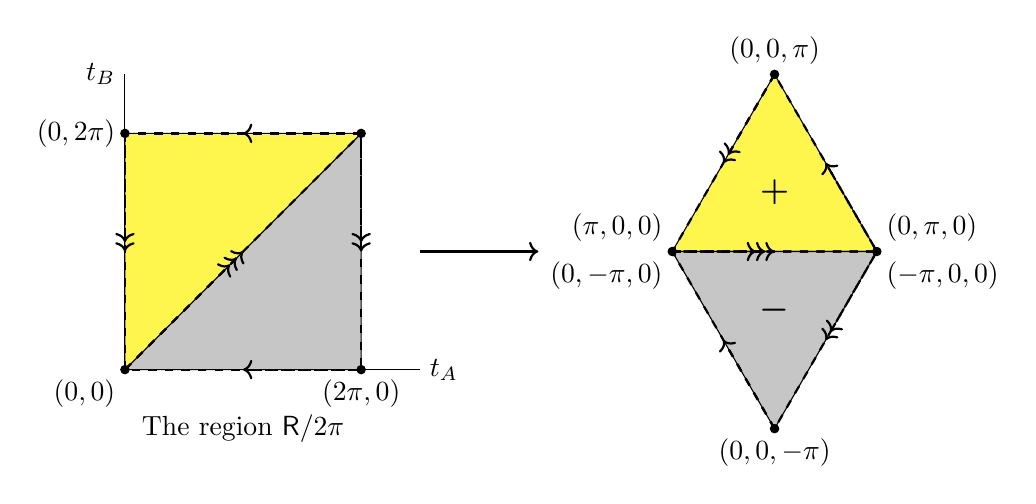
\begin{tikzpicture}[scale=1.5]
%Points
\filldraw (0,0) circle (1pt); %mid bottom
\filldraw (0,2) circle (1pt); %top left
\filldraw (2,2) circle (1pt); %top right
\filldraw (2,0) circle (1pt); %botom right
%\filldraw (1,1) circle (.5pt); %isosceles point in Q_C
%\filldraw (1,2) circle (.5pt); %isosceles point in Q_C
%\filldraw (0,1) circle (.5pt); %isosceles point in Q_C
%Lines
\draw[thick, dashed] (0,0)--(0,2)--(2,2)--(2,0)--(0,0); %perimeter
\draw[thick, dashed] (0,0)--(2,2); %diagonal
\draw (0,0)--(0,2.5); %y-axis.
\draw (0,0)--(2.5,0); %x-axis.
\draw[thick, dashed, ->] (2,2)--(1,2);
\draw[thick, dashed, ->] (2,0)--(1,0);
\draw[thick, dashed, ->>] (0,2)--(0,1);
\draw[thick, dashed, ->>] (2,2)--(2,1);
\draw[thick, dashed, ->>>] (0,0)--(1,1);
\draw[thick, ->] (2.5,1)--(3.5,1);
%Colors
\begin{scope}[on background layer]
\draw[fill=darkgray!30] (0,0)--(2,2)--(2,0)--(0,0); %lower right
\draw[fill=yellow!70] (0,0)--(2,2)--(0,2)--(0,0); %yellow perimeter
%\draw[fill=yellow!100] (1,1)--(1,2)--(0,1)--(1,1); %yellow acute
%\draw[fill=darkgray!50] (1,0)--(1,1)--(2,1)--(1,0); %lower right acute
\end{scope}
%Nodes
\node[left] at (0,2) {$(0,2\pi)$};
\node[below] at (2,0) {$(2\pi,0)$};
\node[below left] at (0,0) {$(0,0)$};
\node[right] at (2.5,0) {$t_A$};
\node[left] at (0,2.5) {$t_B$};
\node at (1,-.5) {The region $\mathsf R/2\pi$};
%%%%%%%%%%%%%%%%%%%%%%%%%%%%%%%%%%%%%%%%%%%%%%%%%%%%
%Points
\filldraw ({5.5+sqrt(3)/2},1) circle (1pt); % right
\filldraw ({5.5+-sqrt(3)/2},1) circle (1pt); % left
\filldraw (5.5,5/2) circle (1pt); %top gold
%\filldraw (5.5,1) circle (.5pt); %bottom foot gold
%\filldraw ({5.5-sqrt(3)/4},7/4) circle (.5pt); %left foot gold
%\filldraw ({5.5+sqrt(3)/4},7/4) circle (.5pt); %right foot gold
%\filldraw ({5.5-sqrt(3)/4},1/4) circle (.5pt); %left foot gray
%\filldraw ({5.5+sqrt(3)/4},1/4) circle (.5pt); %right foot gray
\filldraw (5.5,-1/2) circle (1pt); %bottom gray
%Lines
\draw[thick,dashed] (5.5,5/2)--({5.5-sqrt(3)/2},1)--({5.5+sqrt(3)/2},1)--(5.5,5/2); %perimeter gold triangle
%\draw (5.5,1)--({5.5+sqrt(3)/4},7/4)--({5.5-sqrt(3)/4},7/4)--(5.5,1); %perimeter dark gold
\draw[thick,dashed] (5.5,-1/2)--({5.5-sqrt(3)/2},1)--({5.5+sqrt(3)/2},1)--(5.5,-1/2); %perimater gray
%\draw (5.5,1)--({5.5+sqrt(3)/4},1/4)--({5.5-sqrt(3)/4},1/4)--(5.5,1); %perimeter dark gray
\draw[thick,dashed,->>] (5.5,5/2)--({5.5-sqrt(3)/4},7/4); %gold
\draw[thick,dashed,->>>] ({5.5-sqrt(3)/2},1)--(5.5,1); %gold
\draw[thick,dashed,->] ({5.5+sqrt(3)/2},1)--({5.5+sqrt(3)/4},7/4); %gold
\draw[thick,dashed,->] (5.5,-1/2)--({5.5-sqrt(3)/4},1/4); %gray
\draw[thick,dashed,->>] ({5.5+sqrt(3)/2},1)--({5.5+sqrt(3)/4},1/4);
%Shading
\begin{scope}[on background layer]
%\draw[fill=yellow!100] (5.5,1)--({5.5+sqrt(3)/4},7/4)--({5.5-sqrt(3)/4},7/4)--(5.5,1);
\draw[fill=yellow!70] (5.5,5/2)--({5.5-sqrt(3)/2},1)--({5.5+sqrt(3)/2},1)--(5.5,5/2); 
\draw[fill=darkgray!30] (5.5,-1/2)--({5.5-sqrt(3)/2},1)--({5.5+sqrt(3)/2},1)--(5.5,-1/2);
%\draw[fill=darkgray!50] (5.5,1)--({5.5+sqrt(3)/4},1/4)--({5.5-sqrt(3)/4},1/4)--(5.5,1);
\end{scope}
%nodes
\node[above left] at ({5.5-sqrt(3)/2},1) {$(\pi,0,0)$};
\node[below left] at ({5.5-sqrt(3)/2},1) {$(0,-\pi,0)$};
\node[above right] at ({5.5+sqrt(3)/2},1) {$(0,\pi,0)$};
\node[below right] at ({5.5+sqrt(3)/2},1) {$(-\pi,0,0)$};
\node[above ] at (5.5,5/2) {$(0,0,\pi)$};
\node[below] at (5.5,-1/2) {$(0,0,-\pi)$};
\node at (5.5,1/2) {\large$\boldsymbol -$};
\node at (5.5,3/2) {\large $\boldsymbol +$};
\end{tikzpicture}
\caption{Pairs of Arguments vs. Triples of Angles} 
\label{fig:R/2pi}
\end{figure}